\documentclass[a4paper,10pt]{article}
\usepackage[utf8]{inputenc}
\usepackage{graphicx}
\usepackage{amsmath}

\setlength\textwidth{6.5in}
\setlength\oddsidemargin{0in}
\setlength\evensidemargin{0in}


%\makeatletter
% \renewcommand\paragraph{\@startsection{paragraph}{4}{\z@}%
%   {-3.25ex\@plus -1ex \@minus -.2ex}%
%   {1.5ex \@plus .2ex}%
%   {\normalfont\normalsize\bfseries}}
% \makeatother
% \renewcommand{\thechapter}{}
% \renewcommand \thesection {\arabic {section}}
% Title Page
\title{Architecture of E-Health Flanders platform}
\author{}

%TODO: stijl kiezen: componenten vet, interfaces /...
%TODO: Overal keys toevoegen.
%TODO: afwegingen voor en nadelen.

\begin{document}
\maketitle

\part{Documentation Beyound Views}

\section{Documentation roadmap}

\subsection{Description of the parts}

\subsection{Stakeholders}
De stakeholders waarop dit document zich focust, zijn de patiënt, de tester en de regering.

\paragraph{Patiënt:}
De patiënt wil dat wanneer hij bij zijn huisdokter op consultatie gaat, dat de dokter zijn medisch dossier kan raadplegen en aanpassen. Hiervoor moet de patiënt zijn dokter wel de nodige toelatingen geven. Ook wil de patiënt zelf zijn medisch dossier kunnen raadplegen. 

\paragraph{Tester:}
De tester wil de eHealth applicatie grondig testen en alle mogelijke scenarios uitproberen.

\paragraph{Regering:}
De regering wil kunnen beslissen hoe de toegang tot de medische dossiers wordt geregeld (hoeveel van hun dossier kunnen patiënten zelf zien, welke dokter kan wat aanpassen etc). Ook wil de regering een log kunnen raadplegen waarin alle activiteiten op het eHealth platform gelogd worden. Hieronder vallen onder andere inloggen, medische dossiers raadplegen, medische dossiers aanpassen en voorschriften valideren. Een tak van de regering bestaat uit het RIZIV, die informatie over de uitgeschreven en gevalideerde voorschriften wil bijhouden.

\subsubsection{How stakeholders might use the package}

\paragraph{Patiënt:}
De patiënt gebruikt een client-applicatie om het eHealth platform te raadplegen. Wanneer hij op consultatie is, gebeuren de gewenste acties via de client-applicatie van de dokter. Voor de patiënt is de client-kant van deze applicatie dus belangrijk.

\paragraph{Tester:}
Voor de tester zijn er uitgewerkte sequentiediagrammen aanwezig, die een overzicht geven van hoe de verschillende acties tot stand komen. Daarnaast is in zowel het Client-server diagram als het deployment diagram te zien hoe de verschillende functionaliteiten in afzonderlijke componenten zitten, waardoor het testen van de functionaliteiten afzonderlijk eenvoudig is. Ook het layered view geeft een overzicht van hoe de verschillende componenten samen werken.

\paragraph{Regering:}
Er is een afzonderlijke component voorzien die de functionaliteiten die de regering vereist, uitvoert. Zo worden alle acties gelogd naar een log, buiten het systeem, en ook de boodschappen naar het RIZIV worden via deze component gestuurd. 

\clearpage
\section{View template}

\clearpage
\section{System overview}

\clearpage
\section{Mapping between views}
\label{Mappingbetweenviews}

\clearpage
\section{Directory}

\clearpage
\section{Glossary and acronym list}

\clearpage
\section{Background, design constraints, and rationale}
Veel van de beslissingen die we genomen hebben zijn telkens te vinden in de gedetailleerdere stukken van de architectuur.  Hier proberen we toch enkele algemene architectuur beslissingen te verantwoorden.\\
TODO
%TODO


\part{Software Architecture Views}
\setcounter{section}{0}

\clearpage
\section{Module Layered View: Client}

\subsection{Primary presentation}

\begin{center}
    \begin{figure}[h!]
      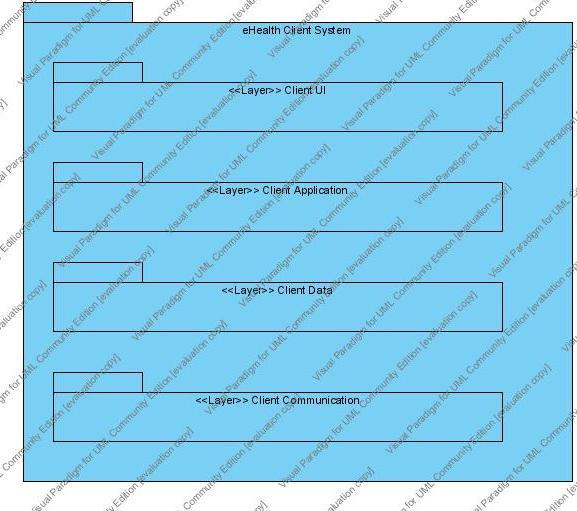
\includegraphics[width=\textwidth]{../images/LayeredView_Client.jpg}
    \end{figure}
  \end{center}

\subsection{Element catalog}

\subsubsection{Elements and their properties}

-Software Layer: naam, verantwoordelijkheid , inhoud\\

Client UI Layer\\

Verantwoordelijkheid:\\
Uiterlijk presentatie van Client Applications.\\

Inhoud:\\
GUI (buiten project scope)\\

Client Application Layer\\

Verantwoordelijkheid:\\
-Implementatie van specifieke business logica.\\
-Validatie van gebruikers identiteit. Enkel bevoegde personene kunnen bepaalde applicatie gebruiken en toegang krijgen tot bijhorende data.\\

Inhoud:\\
GP Application (buiten project scope)\\
Card Reader Module\\

Client Data Layer\\

Verantwoordelijkheid:\\
-Uniformaliteit aanbieden voor de toegang tot data's. In normaal geval moet de gebruiker niet weten waar de data vandaan gehaald wordt, lokale cache of external data server.\\
-Standaard voor- en nabewerkingen uitvoeren op data's: encryptie/decryptie, compressie/decompressie.\\
-Opslaan van lokale data cache en consistentie onderhouden tussen lokale cache en external data server.\\

Inhoud:\\
Data Manager, Cache, Security (Authentication en Compression)\\

Client Communication Layer\\

Verantwoordelijkheid:\\
Communicatie met externe systemen (GMR Server).\\

Inhoud:\\
Network Module (buiten project scope)\\


\subsubsection{Relations and their properties}

-Allowed-to-Use: Layer A en Layer B hebben de relatie "A is allowed-to-use B" als A onmiddellijk boven B staat, tenzijn anders expliciet vermeld.\\

\subsubsection{Element interfaces}

\subsubsection{Element behavior}

\subsection{Context diagram}

\subsection{Variability guide}

\subsection{Architecture background}

\subsubsection{Rationale}

\subsubsection{Analysis results}

\subsubsection{Assumptions}

\subsection{Other information}

\subsection{Related view packets}

Sibling: Layered View: Server\\
Child: Uses View: Client\\


\section{Module Layered View: Server}

\subsection{Primary presentation}
\begin{center}
    \begin{figure}[h!]
      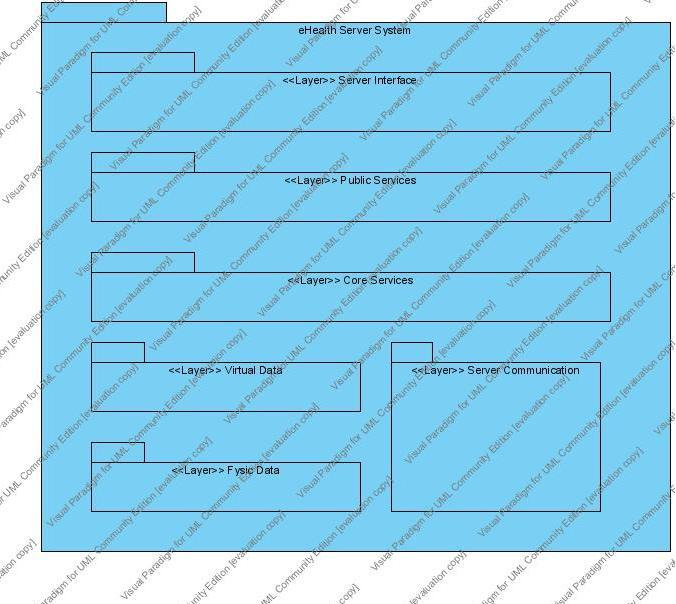
\includegraphics[width=\textwidth]{../images/LayeredView_Server.jpg}
    \end{figure}
  \end{center}

\subsection{Element catalog}

\subsubsection{Elements and their properties}

-Layer: naam, verantwoordelijkheid , inhoud\\

Server Interface Layer\\

Verantwoordelijkheid:\\
Verbindingen van gebruikers ontvangen en delegeren naar Public Services Layer.\\

Inhoud:\\
Proxy\\

Public Services Layer\\

Verantwoordelijkheid:\\
Publiek service ter beschikking stellen voor gebruikers. Aan de hand van gekozen publiek service worden de onderliggende kern service opgeroepen.\\
Op dit niveau wordt zijn de gebruikers nog volledige anoniem.\\

Inhoud:\\
Public Service\\

Core Services Layer\\

Verantwoordelijkheid:\\
Implementatie van business logica van eHealth platform.\\
Basis bouwblokken voorzien voor publoek service.\\
Identificatie van gebruiker en de bevoegdheid van gebruiker controleren.\\

Inhoud:\\
GMR, Security, Session Management, Policy\\

Virtual Data Layer\\

Verantwoordelijkheid:\\
Bescherming van data's tegen onbevoegde toegang.\\
Uniformaliteit aanbieden voor de toegang tot data's.\\

Inhoud:\\
Virtual GMR Data\\

Fysic Data Layer\\

Verantwoordelijkheid:\\
Bescherming van data's tegen data-corruptie.\\
Opslag van Medical Records.\\
Opslag van Security data's die nodig zijn voor Authorization/Authentication van client gebruikers.\\

Inhoud:\\
GMR Data Server, Doctor Data Server, Security Server\\


Server Communication Layer\\

Verantwoordelijkheid:\\
Communicatie met externe systemen (RIZIZ, Log).\\

Inhoud:\\
Network Module (buiten project scope)\\




\subsubsection{Relations and their properties}

-Allowed-to-Use: Layer A en Layer B hebben de relatie "A is allowed-to-use B" als A onmiddellijk boven B staat, tenzijn anders expliciet vermeld.\\

\subsubsection{Element interfaces}

\subsubsection{Element behavior}

\subsection{Context diagram}

\subsection{Variability guide}

\subsection{Architecture background}

\subsubsection{Rationale}

\subsubsection{Analysis results}

\subsubsection{Assumptions}

\subsection{Other information}

\subsection{Related view packets}

Sibling: Layered View: Client\\
Child: Uses View: Server\\

\section{Module Uses View: Client}

\subsection{Primary presentation}
\begin{center}
    \begin{figure}[h!]
      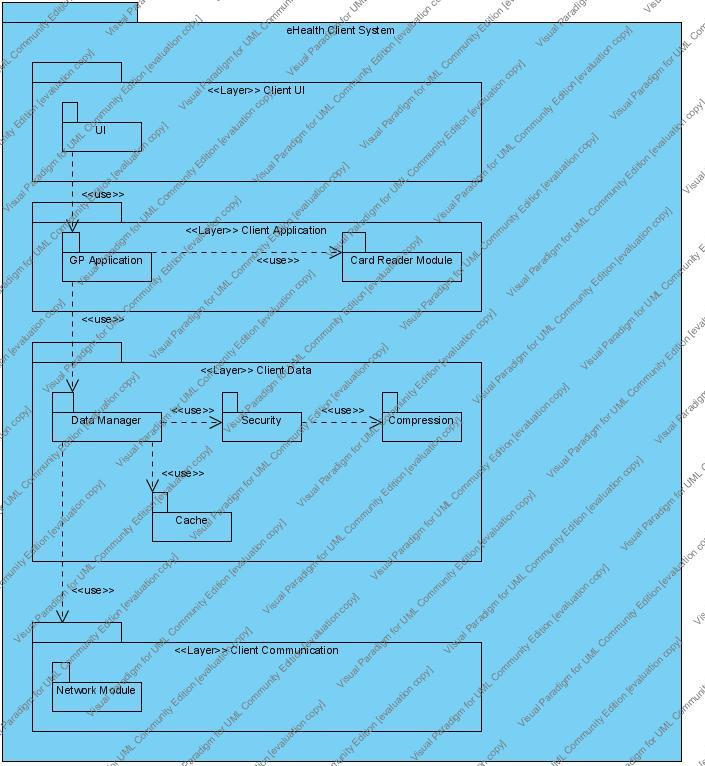
\includegraphics[width=\textwidth]{../images/UsesView_Client.jpg}
    \end{figure}
  \end{center}

\subsection{Element catalog}

\subsubsection{Elements and their properties}

-Software Module: naam, beschrijving\\

GUI\\
Bebruikers interface\\
(buiten project scope)\\

GP application\\
Professionele dokter software applicaties.\\
(buiten project scope)\\

Card Reader Module\\
Besturingssoftware voor Card Reader. Software interface van de hardware, maakt het mogelijk om de Card Reader te gebruiken door andere software applicaties.\\

Data Manager\\
Algemeen data management, camoufleert de exacte lokatie van data's, behandelt basis data bewerkingen en zorgt voor consistentie tussen lokale cache en external server data's.\\

Cache\\
zie C\&C View: Client\\

Security\\
zie C\&C View: Client\\

Compression\\
zie C\&C View: Client\\

Network Module\\
Standaard network software applicaties.\\
(buiten project scope)\\


\subsubsection{Relations and their properties}

- Uses: een layer of een software module will gebruik maken van een andere layer of software module als de eerste expliciet verbonden is met de tweed. Wanneer de tweede entieit een layer is, mogen alle ingesloten software modules gebruikt worden door de eerste entiteit.\\

\subsubsection{Element interfaces}

Interfaces van elementen die getoond worden in dit view worden gespecifieerd door de overeenkomende elementen in Module C\&C View\\

\subsubsection{Element behavior}

\subsection{Context diagram}

\subsection{Variability guide}

\subsection{Architecture background}

\subsubsection{Rationale}

\subsubsection{Analysis results}

\subsubsection{Assumptions}

\subsection{Other information}

\subsection{Related view packets}

Sibling: Uses View: Server\\
Parent: Layered View: Client\\

\section{Module Uses View: Server}

\subsection{Primary presentation}
\begin{center}
    \begin{figure}[h!]
      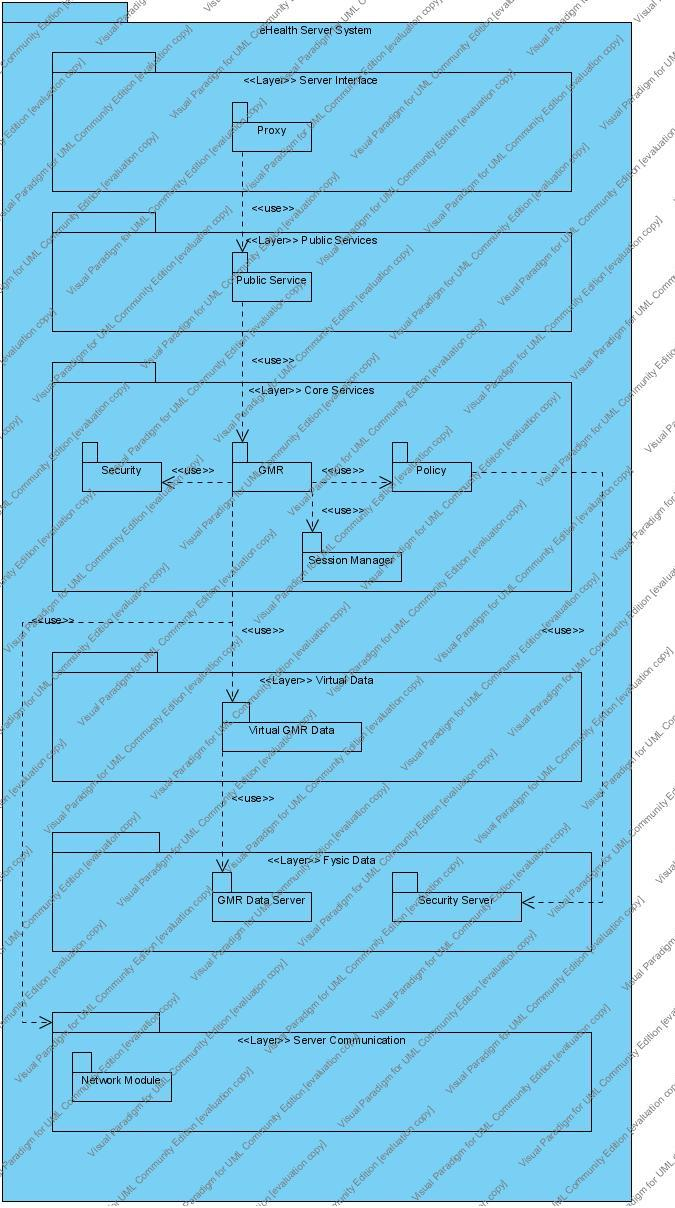
\includegraphics[height=\textheight]{../images/UsesView_Server.jpg}
    \end{figure}
  \end{center}

\subsection{Element catalog}

\subsubsection{Elements and their properties}

Proxy\\
zie Deployment View\\

Public Service\\
zie Deployment View\\

GMR\\
zie C\&C View\\

Security\\
zie C\&C View\\

Policy\\
zie C\&C View\\

Session Manager\\
zie C\&C View\\

Virtuam GMR Data\\
zie Deployment View\\

Virtual GMR Data\\
zie Deployment View\\

Security Server\\
zie Deployment View\\

Network Module\\
Standaard network software applicaties.\\
(buiten project scope)\\


\subsubsection{Relations and their properties}

- Uses: een layer of een software module will gebruik maken van een andere layer of software module als de eerste expliciet verbonden is met de tweed. Wanneer de tweede entieit een layer is, mogen alle ingesloten software modules gebruikt worden door de eerste entiteit.\\

\subsubsection{Element interfaces}

Interfaces van elementen die getoond worden in dit view worden gespecifieerd door de overeenkomende elementen in Module C\&C View\\

\subsubsection{Element behavior}

\subsection{Context diagram}

\subsection{Variability guide}

\subsection{Architecture background}

\subsubsection{Rationale}

\subsubsection{Analysis results}

\subsubsection{Assumptions}

\subsection{Other information}

\subsection{Related view packets}

Sibling: Uses View: Client\\
Parent: Layered View: Server\\




\clearpage
\section{C\&C Client and Server View: Overview}
\label{Client and Server View: Overview}

\subsection{Primary presentation}

\begin{figure}[!ht]
  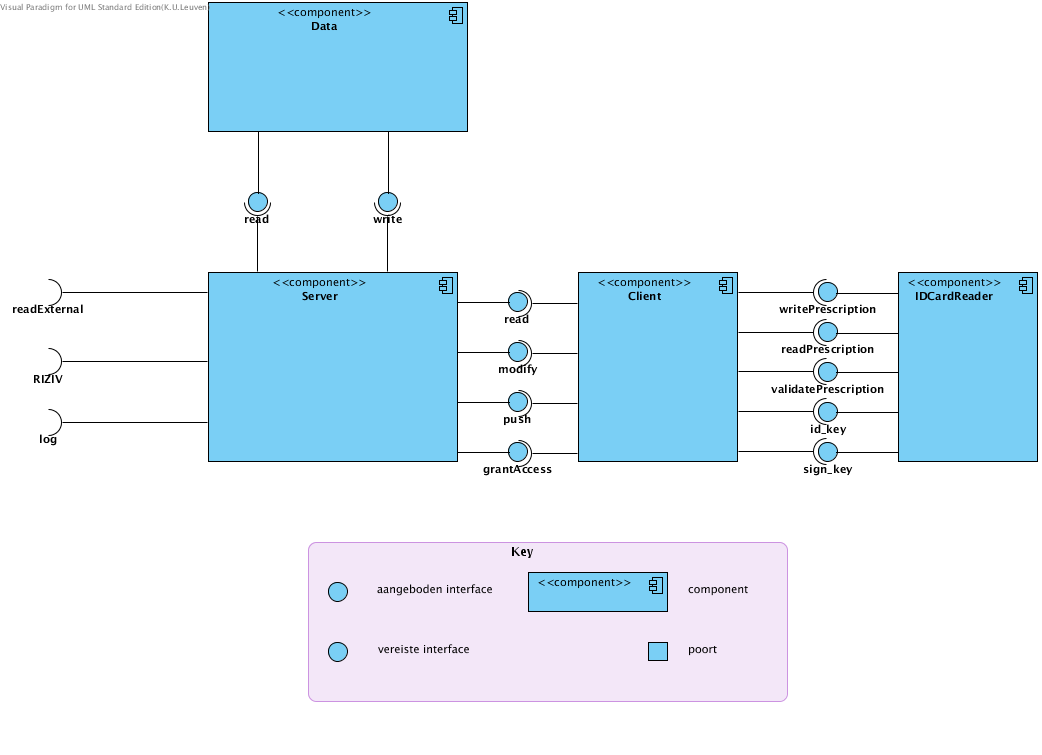
\includegraphics[width=\textwidth]{../images/ClientServer_Overview.png}
  \caption{Client and Server View: Overview}
\end{figure}
%TODO In de figuur die hierboven staat een fout in de legende, bij vereiste interface staat het symbool van een aangeboden interface.

\subsection{Element catalog}

\paragraph{Server}
De server is de component waar clients verbinding mee maken.  De interacties tussen clients en servers gebeuren op een veilige manier.  De server is verbonden met clients, de overheid, eventuele externe componenten en de data server.  Meer informatie kan gevonden worden in \ref{Client and Server View: Server} Client and Server View: Server.

\paragraph{Client}
De client component is de component die gebruikers (dokters, pati\"{e}nten of apothekers) gebruiken om op een veilige manier met de server te interageren.  Meer informatie kan gevonden worden in \ref{Client and Server View: Client} Client and Server View: Client.

\paragraph{Data}
De data component is een database waar alle informatie zoals patienten dossiers en dokter data op bewaard zijn.  Hoe de data precies wordt opgeslaan is terug te vinden in het \ref{sec:deployment_data} Deployment view data.
%TODO read write interfaces?

\paragraph{Card}
De card component stelt de e-Card van de gebruiker voor.  De e-Card bevat gebruikersinformatie alsook twee keys.  Een key voor identificatie van de gebruiker en een key voor authenticatie.  Naast de gebruikersinformatie en de keys heeft de e-Card ook ruimte voor een aantal voorschriften op te slaan.  Meer informatie is terug te vinden in: TODO alsook in enkele interactie diagramma's (zie: \ref{interaction:addPrescription} en \ref{interaction:validatePrescription}).
%TODO location
%TODO interfaces van card

\subsection{Context diagram}

\begin{figure}[!ht]
  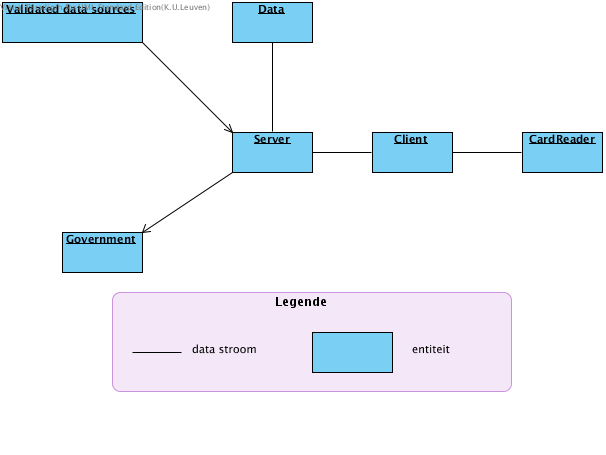
\includegraphics[width=\textwidth]{../images/ClientServer_Context.png}
  \caption{Client and Server View: Context diagram}
\end{figure}

De belangrijkste extra entiteiten in het context diagram zijn de government en de validated data sources.  De government component bevat toegang tot de logging en RIZIV database.  De validated data sources kunnen gebruikers van de client opvragen via de server.

\subsection{Variability guide}
[None]

\subsection{Architecture background}
De meeste archituur achtergrond is te vinden in gedetailleerdere views waar reeds eerder naar verwezen is.  De algemene structuur is hier wel duidelijk waarbij de Client kant met behulp van de e-Card zich in het systeem kan identifici\"{e}ren (zie ook \ref{Client and Server View: Security} Client and Server View: Security).  Aan de andere kant is de server te vinden die zorgt voor veilige opslag en toegang tot de data en tot andere externe bronnen (zie ook \ref{Client and Server View: Server} Client and Server View: Server).
%TODO voorschriften.

\subsection{Related view packets}
De volgende client-server views bekijken dit overview diagram in meer detail.  Ook in het deployment diagram is extra informatie te vinden vooral dan in verband met de opslag van de global medical records en dokter data.



\clearpage
\section{C\&C Client and Server View: Server}
\label{Client and Server View: Server}
\subsection{Primary presentation}

\begin{figure}[!ht]
  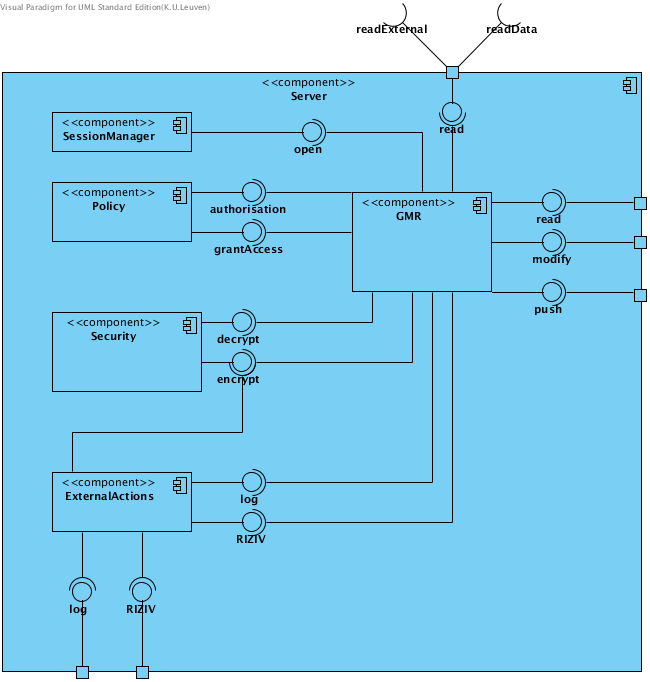
\includegraphics[scale=0.60]{../images/ClientServer_Server.png}
  \caption{Client and Server View: Server}
\end{figure}

\subsection{Element catalog}

\paragraph{GMR}
De GMR is de centrale component in de server component.  De GMR delegeert alle inkomende \textit{read}, \textit{modify} of \textit{push} acties naar de correcte andere componenten en doet dit uiteraard in de correcte volgorde.\\
Om alle interacties beter te begrijpen kunnen de Sequence diagrams vaak ook nuttig zijn (zie: \ref{interaction:main}).

\subsubsection{Element interfaces} 

\paragraph{read}

\underline{Resources provided:}\\
read(data\_key, id\_key)\\
\indent De id\_key wordt geauthenticeerd en daarna wordt een sessie geopent.  De session\_key wordt samen met data die bij de data\_key hoort teruggegeven.\\
read(data\_key, session\_key)\\
\indent De data met data\_key wordt gelezen en teruggeven aan het systeem.\\
%TODO Hierboven misschien ook vermelden dat de data die teruggegeven wordt geëncrypteerd wordt met de id_key.

\underline{Error handling:}\\
Wanneer de data\_key niet geldig is wordt een error teruggegeven.\\
Wanneer de id\_key of session\_key geen toegang heeft tot data\_key wordt een error teruggegeven.\\
Wanneer de id\_key of session\_key niet geldig is wordt een error teruggegeven.\\

\underline{Element requirements:}\\
data\_key: de key om de data op te vragen.\\
id\_key: de key die gebruikt wordt om de uitvoerder van de actie op te vragen.\\
session\_key: de key die gebruikt wordt om een sessie te identifici\"{e}ren.\\

\underline{Rationale and design issues:}\\
Het openen van een sessie wanneer de eerste actie wordt uitgevoerd met een id\_key kan ook aangepast worden om een expliciete login te doen.  Dan zou de client eerst moeten inloggen met de id\_key en dan kan hij later acties uitvoeren met de session\_key.\\
Voor bepaalde acties kan men verwachten dat altijd een id\_key wordt meegegeven.\\
Zie ook \ref{sec:deployment_data} Deployment view data voor het ophalen van data.  Textuele data wordt altijd eerst teruggegeven, daarna pas andere data (media bestanden zoals figuren, geluid, video).

\paragraph{modify}
\underline{Resources provided:}\\
modify(data\_key, data, id\_key)\\
modify(data\_key, data, session\_key)\\
Het inloggen en valideren gebeurt zoals beschreven bij \textbf{read}.
De aanpassing van de data verloopt door het mergen van data met de bestaande data.  Wanneer de GMR een antwoord krijgt van de database dat alles correct is geschreven verstuurt de GMR een antwoord naar de client dat alle data correct is geschreven.  Deze handelingen gebeuren asynchroon.

\underline{Error handling:}\\
Gelijkaardige errors zoals bij \textbf{read}.\\
Wanneer het mergen van de data faalt zal een error teruggegeven worden.

\underline{Element requirements:}\\
data\_key: de key om de data op te vragen.\\
data: een patch van data die moet aangepast worden op locatie data\_key.\\ 
id\_key: de key die gebruikt wordt om de uitvoerder van de actie op te vragen.\\
session\_key: de key die gebruikt wordt om een sessie te identifici\"{e}ren.\\

\underline{Rationale and design issues:}\\
Zie ook \textbf{read}.\\
Het schrijven van data gebeurt met behulp van een patch, enkel de wijzigingen worden dus doorgestuurd.  Dit verkleint de hoeveelheid data die moet verstuurd worden aanzienelijk en heeft dan ook een belangrijk snelheids voordeel.\\
In het geval dat een merge actie zou falen, kan aan de laatste client gevraagd worden om de merge manueel te doen, of om een volledig document te verzenden.

\paragraph{push}
\underline{Resources provided:}\\
push(data\_key, data, id\_key)\\
push(data\_key, data, session\_key)\\
Het inloggen en valideren gebeurt zoals beschreven bij \textbf{read}.
Het pushen van de data gebeurt gelijkaardig zoals bij \textbf{modify}.

\underline{Error handling:}\\
Gelijkaardige errors zoals bij \textbf{read}.\\

\underline{Element requirements:}\\
data\_key: de key om de data op te vragen.\\
data: data die moet toegevoegd worden aan document met key: data\_key.\\
id\_key: de key die gebruikt wordt om de uitvoerder van de actie op te vragen.\\
session\_key: de key die gebruikt wordt om een sessie te identifici\"{e}ren.\\

\underline{Rationale and design issues:}\\
Zie ook \textbf{read}.\\
Hier kan geen patch gestuurd worden omdat een push actie enkel toelaat nieuwe data toe te voegen aan een dossier.\\
Alhoewel push ongeveer gelijkaardig is aan modify hebben we er toch voor gekozen om deze toe te voegen.  Met behulp van push kunnen bepaalde personen toch toegang krijgen tot het schrijven van data bij een dossier zonder dat dossier te kunnen lezen.

\paragraph{grantAccess}
\underline{Resources provided:}\\
grantAccess(to\_key, data\_key, action, from\_key, period)\\
Zie grantAccess bij \textbf{Policy}.  Daar wordt de interface uitgewerkt, de interface hier wordt gewoon gedelegeert naar de interface van \textbf{Policy}.

\subsubsection{Element behavior}
De GMR component delegeert alle inkomende acties.  Dat doet hij door inkomende berichten door de security component te laten decrypten.  Dan krijgt hij onmiddellijk bevestiging dat de data compleet en correct is en van de een geauthenticeerde gebruiker komt.  Indien dit niet het geval is stuurt de GMR een error terug naar de client.\\
Daarna wordt gecontroleerd of er al een sessie bestaat en of die al dan niet geldig is.\\
Wanneer dat gebeurd is zal het systeem de oproep doorgeven aan de policy component.  Deze zal de GMR laten weten of de actie die de GMR binnen krijgt al dan niet toegelaten is.\\
Als de actie toegelaten is voor de gebruiker zal de GMR de actie uitvoeren en een gepaste respons sturen naar de client.\\
Als het nodig is worden acties gelogd of verzonden naar het RIZIV.\\
(Het gedrag dat hier beschreven is komt niet volledig overeen met het deployment model.  Zie \ref{Mappingbetweenviews} Mapping between views en \ref{sec:deployment_services} Deployment view services.)


\paragraph{SessionManager}
De SessionManager voorziet in session management.  Deze component zorgt ervoor dat een gebruiker niet telkens opnieuw hoeft in te loggen wanneer hij een actie naar het systeem uitvoert.

\subsubsection{Element interfaces} 

\paragraph{open}
\underline{Resources provided:}\\
open(id\_key)\\
Opent een nieuwe sessie voor id\_key, de session\_key wordt teruggegeven.

\underline{Element requirements:}\\
id\_key: de key waarmee de client zich identifici\"{e}ert.

\underline{Rationale and design issues:}\\
Voorziet in het openen van sessies, waardoor de client niet telkens zijn identificatie key moet opnieuw ingeven.

\paragraph{valid}
\underline{Resources provided:}\\
valid(session\_key)\\
Dit controleert of de session\_key nog geldig is, een sessie verloopt na een bepaalde tijd.  Er wordt teruggeven als de session\_key nog al dan niet geldig is.  Als ze nog geldig is wordt de id\_key teruggegeven die verbonden is met deze session\_key.

\underline{Element requirements:}\\
session\_key: de key die gebruikt wordt om een sessie te identifici\"{e}ren.\\

\underline{Rationale and design issues:}\\
Hoe lang een sessie geldig blijft zou kunnen aangepast worden afhankelijk van wie er in het systeem inlogt of afhankelijk van welke soort client.  Wanneer de client toepassing op een smartphone draait zou er kunnen gekozen worden om de session\_keys sneller te laten vervallen aangezien deze omgeving als minder veilig kan beschouwt worden.  Indien we dit willen afdwingen moet wat extra informatie worden meegegeven bij het openen van de sessie.

\subsubsection{Element behavior}
De SessionManager is verantwoordelijk voor het openen van sessies (\textit{open}) en het controleren of een bepaalde sessie geldig is (\textit{valid}).

\paragraph{Policy}
Deze component controleert de toegangsrechten van de gebruikers en laat weten welke gebruikers toegang hebben tot welke delen van de data en wat die toegang inhoudt (lezen en of schrijven).

\subsubsection{Element interfaces} 

\paragraph{autorisation}
\underline{Resources provided:}\\
authorize(data\_key, action, id\_key)\\
De authorisatie component kijkt of de persoon met identificatie id\_key toelating heeft om actie action uit te voeren op document met key data\_key.  Er wordt teruggegeven of de actie al dan niet is geauthoriseerd.

\underline{Element requirements:}\\
data\_key: de key verbonden met een data document.\\
action: een actie die uitgevoerd zal worden, dit kan read, modify of push zijn.\\
id\_key: de key die de uitvoerder van de actie identifici\"{e}ert.\\

\underline{Rationale and design issues:}\\
De autorisation component keurt de toegang goed voor personen die eerder toegang verkregen hebben tot iets via grantAccess (zie hieronder).

\paragraph{grantAccess}
\underline{Resources provided:}\\
grantAccess(to\_key, data\_key, action, from\_key, period)\\
De persoon verbonden aan from\_key geeft toegangrechten voor periode period aan to\_key om actie action uit te voeren op het document met key data\_key.

\underline{Error handling:}\\
De persoon met from\_key heeft geen toelating de toegangsrechten voor actie action toe te kennen.\\
De persoon met to\_key kan geen toegangsrechten krijgen om actie action uit te voeren.\\

\underline{Element requirements:}\\
to\_key: de identificatie key van de persoon aan wie toegangsrechten worden toegekend.
data\_key: de key verbonden met een data document.\\
action: een actie waarvoor rechten worden uitgedeeld.  Action kan hier ook zijn het toekennen van toegangsrechten aan een andere persoon.
from\_key: de identificatie key van de persoon die de toegangsrechten uitdeelt.
period: de periode hoe lang de persoon met to\_key toegang krijgt tot de data.

\underline{Rationale and design issues:}\\
Door de grantAccess toe te voegen kunnen toegangsrechten worden toegekend aan andere personen en kan dit voor een bepaalde tijdsduur.  Action is hier niet enkel read, modify of push zodat bepaalde personen ook toelating krijgen om toegangsrechten door te geven.  Zo zou een specialist bijvoorbeeld ook toegang kunnen krijgen om read toegang tot het dossier ook door te geven aan een andere specialist.\\
Zie ook \ref{interaction:grantAccess} Interaction diagram: grant access.

\subsubsection{Element behavior}
De policy component zal authorisatie toekennen aan bepaalde acties, als die persoon de actie mag uitvoeren.  Indien dat niet mag zal de authorisatie geweigerd worden.  Bepaalde personen hebben ook rechten om nieuwe rechten toe te voegen.  Deze worden via \textit{grantAccess} toegevoegd.  In de interactie diagramma's is het verloop duidelijk te volgen (zie \ref{interaction:grantAccess}).

\paragraph{Security}
De gedetailleerde uitwerking van de security component is te vinden in \ref{Client and Server View: Security} Client and Server View: Security.

\paragraph{ExternalActions}

\subsubsection{Element interfaces} 
De Element interface component voorziet de interfaces voor het loggen naar de overheid en het verzenden van de RIZIV data naar de overheid.

\paragraph{log}
\underline{Resources provided:}\\
log(data)\\
De data wordt gelogd naar de overheid toe.  De component zorgt dat enkel data die mag gelogd worden verstuurd wordt.

\underline{Element requirements:}\\
data: de data om te loggen.

\underline{Rationale and design issues:}\\
De data die mag gelogd worden kan eventueel gedefinieerd worden door een externe instantie, in dit geval de overheid.
Zie ook \ref{sec:deployment_services} Deployment view services voor toegang tot de overheid.

\paragraph{RIZIV}
\underline{Resources provided:}\\
riziv(data)\\
De data wordt verzonden naar de overheid toe.  De component zorgt data alle data die moet verzonden worden, verzonden wordt.

\underline{Error handling:}\\
Wanneer de data niet volledig is wordt een error teruggeven.

\underline{Element requirements:}\\
data: de data om te verzenden naar het RIZIV.

\underline{Rationale and design issues:}\\
Zie ook \ref{sec:deployment_services} Deployment view services voor toegang tot de overheid.

\subsubsection{Element behaviour}
Deze component zal de logging en RIZIV acties uitvoeren naar de overheid toe.  In normale omstandigheden zullen deze acties onmiddellijk uitgevoerd worden.  In het geval dat de server van de overheid niet kan bereikt worden zullen de acties gequeued worden totdat de server terug beschikbaar is.  Op het moment dat de server opnieuw beschikbaar is zal de queue element per element verzonden worden naar de overheid.\\
Deze queue kan anders uitgewerkt worden voor log en RIZIV.

\subsection{Context diagram}
Het \ref{Client and Server View: Overview} Client and Server View: Overview diagram kan beschouwd worden als het context diagram voor de server.

\subsection{Variability guide}
Het inloggen het systeem gebeurt nu impliciet.  Op het moment dat de \textbf{GMR} een actie binnen krijgt met een id\_key zal aan de \textbf{SessionManager} gevraagd worden om een nieuwe sessie te openen.  Dan zal de sessie\_key teruggegeven worden aan de gebruiker.  Dit kan ook aangepast worden om expliciet een login te vereisen voordat de eerste actie in het systeem wordt uitgevoerd.\\
De \textbf{ExternalActions} component kan ook zo uitgewerkt worden dat de acties slechts op bepaalde tijdstippen naar de server van de overheid worden uitgevoerd.  De acties worden dan altijd gequeued.  Op bepaalde tijdstippen worden de queues dan uitgevoerd en leeggemaakt.  Er zou ook kunnen rekening gehouden worden met het aantal elementen in de queue.  De queue kan dan worden uitgevoerd en leeggemaakt als een bepaalde treshold van elementen bereikt is.  Tenslotte is ook een combinatie van beide vorige mogelijk.  De queue kan normaal op een bepaald tijdstip leeggemaakt worden tenzij er te veel elementen in de queue zitten; dan zou de queue eerder worden geleegd.  Omgekeerd kan het ook dat de queue altijd geleegd worden zodra een bepaald elementen in de queue zitten, maar ook op bepaalde tijdstippen om in het geval van low traffic de berichten niet te lang op de server te houden.\\
Het is mogelijk verschillende instellingen te gebruiken voor log en RIZIV.\\
Het is ook mogelijk om de interfaces zo te implementeren dat bepaalde berichten een hogere prioriteit hebben en altijd direct worden verzonden naar de overheid.

\subsection{Architecture background}
We hebben de \textbf{Server} zo gemaakt met een centrale component die alle delegatie doet; de \textbf{GMR}.  De \textbf{GMR} heeft zelf wel geen verantwoordelijkheden buiten het delegeren van alle inkomende acties.

\subsection{Other information}
[None]

\subsection{Related view packets}
In \ref{sec:deployment_data}, het Deployment view data is te zien hoe de connection naar de externe servers tot stand komt.\\
In de interactie diagramma's (zie \ref{interaction:main} zijn ook voorbeelden te vinden van hoe bepaalde interacties precies in hun werk gaan.


\clearpage
\section{C\&C Client and Server View: Client}
\label{Client and Server View: Client}

\subsection{Primary presentation}

\begin{figure}[!h]
  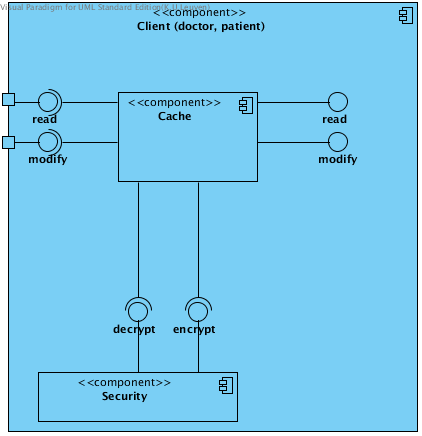
\includegraphics[width=70mm]{../images/ClientServer_Client.png}
  \caption{Client and Server View: Client}
\end{figure}

\subsection{Element catalog}

\paragraph{Cache}
De cache component is een lokale cache van bestanden die ook op de server of externe servers aanwezig zijn.  Dit element voorziet de toegang tot de data.

\subsubsection{Element interfaces} 

\paragraph{read}

\underline{Resources provided:}\\
read(data\_key)\\
De data verbonden met data\_key wordt gelezen (zie ook Elemenet behavior).

\underline{Element requirements:}\\
data\_key: de key om de data op te vragen.\\

\underline{Rationale and design issues:}\\
Zie hieronder voor een beschrijving van het algemeen gedrag van de cache.

\paragraph{modify}
\underline{Resources provided:}\\
modify(data\_key, data)\\
De aanpassing van de data verloopt door het mergen van data met de bestaande data (zie ook Elemenet behavior).

\underline{Error handling:}\\
Wanneer het mergen van de data faalt zal een error teruggegeven worden.  Er kan gevraagd worden aan de uitvoerder van de actie om manueel een merge uit te voeren.

\underline{Element requirements:}\\
data\_key: de key om de data op te vragen.\\
data: een patch van data die moet aangepast worden op locatie data\_key.\\ 

\underline{Rationale and design issues:}\\
In het geval dat een merge actie zou falen, kan aan de client gevraagd worden om de merge manueel te doen, of om een volledig document te verzenden.

\paragraph{push}
\underline{Resources provided:}\\
push(data\_key, data)\\
Het pushen van de data gebeurt gelijkaardig zoals bij \textbf{modify}  (zie ook Elemenet behavior).

\underline{Element requirements:}\\
data\_key: de key om de data op te vragen.\\
data: data die moet toegevoegd worden aan document met key: data\_key.\\

\underline{Rationale and design issues:}\\
Hier kan geen patch gestuurd worden omdat een push actie enkel toelaat nieuwe data toe te voegen aan een dossier.

\subsubsection{Element behavior}
Wanneer een item uit de cache gelezen wordt (\textit{read}), verstuurt de cache eerst de vraag naar de server als het gegeven item up-to-date is.  Als dit het geval is dan wordt het bestand uit de cache aan de gebruiker weergegeven, is dit niet het geval dan stuurt de server het meest recente bestand terug.  Dit wordt dan opgeslagen in de cache en dan teruggegeven aan de gebruiker.\\
%TODO teruggeven aan de gebruiker??
Het schrijven van een item (\textit{write}) gebeurt door het item eerst lokaal te schrijven, daarna verstuurt de cache een write operatie naar de server.  Deze write operatie verloopt door enkel een patch te sturen van de nieuwe data, het volledige document wordt dus niet weggeschreven maar enkel de wijzigingen.  Wanneer de cache een antwoord gekregen heeft van de server dat de schrijfoperatie correct verlopen is mag de cache het geschreven item uit de cache verwijderen.\\
Een \textit{push} operatie is gelijkaardig aan de schrijf operatie van hierboven.  Het enige verschil is dat het in het geval van een \textit{push} gaat over een operatie waarbij de gebruiker geen toegang heeft tot het te schrijven document.  Hij kan enkel een data-veld toevoegen, een veld wijzigen of overschrijven is niet mogelijk.\\
Een laatste belangrijk iets is hoe de cache moet reageren in verband met het falen van het netwerk.  Indien de cache geen reactie krijgt van het netwerk mag hij de lokale files teruggeven.  In het geval dat deze cache gegevens oud zijn kan dit aan gebruiker gemeld worden.  Op het moment dat de cache de server terug kan bereiken zal hij zijn wijzigingen gaan opslaan.  Hiervoor wordt een merge algoritme gebruikt.

\paragraph{Security}
De security component is op zich gelijk aan deze in de server.  De gedetailleerde uitwerking is te vinden in \ref{Client and Server View: Security} Client and Server View: Security.

\subsection{Context diagram}
Het \ref{Client and Server View: Overview} Client and Server View: Overview diagram kan beschouwd worden als het context diagram voor de client.

\subsection{Variability guide}
Verschillende implementaties van de Client component zijn mogelijk.  Wanneer de client lokaal op een pc wordt uitgewerkt voor een dokter zal de cache waarschijnlijk zo veel mogelijk data bijhouden.\\
Voor een client van de dokter die bijvoorbeeld op een smartphone draait is het onrealistisch om te verwachten dat deze alle data zal cachen.  De client kan dan bijvoorbeeld zo uitgewerkt worden dat de cache van de smartphone iedere morgen voor de huisbezoeken gesynct wordt met de nodige pati\"{e}nten van die dag.\\
De centrale pc van de dokter kan een gelijkaardige synchronisatie techniek implementeren voor geplande bezoeken van pati\"{e}nten.\\
Nog een ander geval is het geval van de client voor de apotheek of voor de pati\"{e}nt.  In het geval van een client voor de pati\"{e}nt zal de cache enkel het dossier van de pati\"{e}nt zelf bijhouden.  Voor de apotheek hoeft de cache helemaal geen data te cachen.\\
Een laatste geval is wanneer de cache op een webclient draait.  In dit geval kan de caching aangepast worden naar de mogelijkheden van de webserver.  Hier moet dan wel rekening gehouden worden met de wetgeving die centrale opslag van pati\"{e}nten data verbiedt.  Het is mogelijk dat een webserver zoveel zou gaan cachen dat dit zou kunnen gezien worden als een centrale opslag.  Omdat dit niet toegelaten is moet men er bij de implementatie van deze cache rekening mee houden.  De cache zou zo kunnen aangepast worden om slechts een bepaald aantal documenten bij te houden of enkel de documenten die in een bepaalde tijdspanne opgevraagd zijn.\\
Het schrijven van de cache naar de server kan ook per client ingesteld worden.  Er kan na iedere schrijf actie naar de server geschreven worden, er kan geschreven worden als een dossier wordt gesloten.  Het is ook mogelijk dat de server tijdelijk niet beschikbaar is, dan worden alle schrijfacties in een queue gezet en die kunnen dan geschreven worden op het moment dat de server terug beschikbaar is.

\subsection{Architecture background}
De belangrijkste component van de client, de cache, is gekozen om een aantal redenen.  De eerste is het verzorgen van \texttt{availability}.  Wanneer er een netwerk failure is kan een dokter nog aan alle data die lokaal in de cache zit.  In het geval dat de client een dokter is met een lokale pc zal deze cache waarschijnlijk vrij compleet zijn en ook up to date zijn, zeker wanneer het gaat om geplande bezoeken, aangezien de cache voordien al kan synchronizeren met de server.\\
Een ander belangrijke kwaliteitsvereiste die we hier niet mogen vergeten is de \texttt{performance}.  Een lokale cache zal een belangrijke snelheids winst opleveren aangezien een stuk minder data over het netwerk moet verzonden worden.\\
Het wegschrijven van de wijzigingen in plaats van het volledige document bij een \textit{write} operatie naar de server zorgt ook voor een belangrijke snelheids winst.  Op deze manier zal veel minder data over het netwerk moeten worden verstuurd.

\subsection{Other information}
[None]

\subsection{Related view packets}
Deze client kant moet gezien worden in de volledige overview (zie \ref{Client and Server View: Overview} Client and Server Overview.  Daarnaast is ook het Deployment view (\ref{sec:deploymentView:DMZ}, \ref{sec:deployment_clients}, \ref{sec:deployment_services}, \ref{sec:deployment_data}) belangrijk.


\clearpage
\section{C\&C Client and Server View: Security}
\label{Client and Server View: Security}

\subsection{Primary presentation}
De security component bevind zich zowel in de server als in de client. Deze zorgt voor een veilige communucatie tussen beide.

\begin{figure}[!h]
  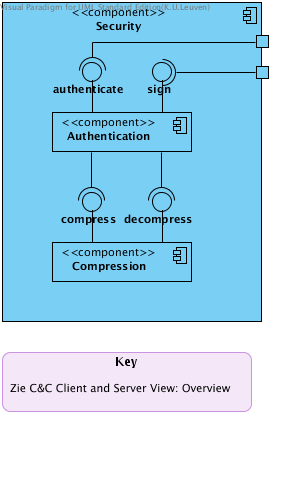
\includegraphics[width=60mm]{../images/ClientServer_Security.png}
  \caption{Client and Server View: Security}
\end{figure}

\subsection{Element catalog}

\paragraph{Authentication}
In deze component wordt de identificatie van de personen die zich inloggen op het systeem gecontroleerd. Wanneer iemand een aanvraag doet, wordt nagegaan of de id\_key van deze persoon overeenkomt met een gebruiker van het systeem. Ook wanneer een boodschap (aanpassen van GMR bv) wordt verstuurd, wordt deze getekend met de key van de zender. Hiervoor dient de sign-interface.  

\subsubsection{Element interfaces}
\paragraph{identify}

\underline{Resources provided:}\\
identify(id\_key)\\
De gebruiker gelinkt met de opgegeven id\_key wordt opgezocht en teruggegeven (zie ook Elemenet behavior).

\underline{Element requirements:}\\
id\_key: de persoonlijke identificatiekey van de gebruiker.\\

\underline{Rationale and design issues:}\\
Wanneer een gebruiker toegang wil tot het systeem, moet hij dit mogen doen. Hiervoor moet zijn identiteit gekend zijn in het systeem. Door zijn persoonlijke identificatiesleutel op te geven, maakt hij duidelijk dat hij is wie hij beweert te zijn en kan het systeem hem identificeren.\\

\paragraph{sign}

\underline{Resources provided:}\\
sign(id\_key)\\
wanneer de gebruiker een boodschap wil versturen, signeert hij de boodschap via deze methode (zie ook Elemenet behavior).

\underline{Element requirements:}\\
id\_key: de persoonlijke identificatiekey van de gebruiker.\\

\underline{Rationale and design issues:}\\
Wanneer de gebruiker een boodschap wil sturen, moet de zender ervan kunnen achterhaald worden. Door de boodschap te signeren met de sign-methode, is de zender ervan bekend bij het systeem en kan achterhaald worden of deze de juiste rechten heeft om deze boodschap uit te voeren.\\

\paragraph{Compression}
Boodschappen die tussen de Client en de Server worden verstuurd, worden gecomprimeerd om tijd te besparen en om een extra vorm van beveiliging toe te voegen.

\subsubsection{Element interfaces}

\paragraph{compress}

\underline{Resources provided:}\\
compress()\\
De boodschap die wordt verstuurd, wordt gecompresseerd zodat deze onleesbaar wordt voor iemand die deze niet kan decompresseren en zodat de grootte van de boodschap wordt verkleind  (zie ook Elemenet behavior).

\underline{Element requirements:}\\
/\\

\underline{Rationale and design issues:}\\
Door de boodschappen die worden verstuurd te compresseren, wordt de boodschap zowel beveiligd, als verkleind, waardoor ook de verzendtijd wordt verkleind.\\

\paragraph{decompress}

\underline{Resources provided:}\\
decompress()\\
Een boodschap die werd verstuurd en gecompresseerd, moet eveneens worden gedecompresseerd om leesbaar te zijn (zie ook Elemenet behavior).

\underline{Element requirements:}
[None]

\underline{Rationale and design issues:}\\
Zie ook compress.\\

\subsubsection{Element behavior}
Deze component zorgt dat de communicatie tussen het platform en de clients veilig verloopt. Enerzijds door de boodschap te signeren met een gebruiker zijn identificatiesleutel, waar het enkel geldige sleutels wordt toegelaten deze boodschappen te sturen. Anderzijds door de boodschappen die verzonden worden te comprimeren. Dit laatste biedt naast veiligheid ook een manier om de communicatie tussen beide te versnellen.\\

\subsection{Context diagram}
De \ref{Client and Server View: Server} Client and Server View: Server en \ref{Client and Server View: Client} Client and Server View: Client diagramma's kunnen beschouwd worden als context diagram voor de security component.

\subsection{Variability guide}
De implementatie van zowel de Authentication component als de compression component zal gebeuren met third-party software. Dit is gemakkelijker dan zelf zo een systeem maken en doordat de componenten zo afgezonderd zijn van het systeem, is het later ook gemakkelijk om een nieuw algoritme te voorzien.\\

\subsection{Architecture background}

\subsubsection{Rationale}
zie Element behavior.
%TODO 2 keys => qualities.


\subsection{Other information}
[None]

\subsection{Related view packets}
De security component is zowel in de client (\ref{Client and Server View: Client} Client and Server View: Client) als de server (\ref{Client and Server View: Server} Client and Server View: Server) component te zien.

\clearpage
\section{Deployment view DMZ}
\label{sec:deploymentView:DMZ}

\subsection{Primary presentation}
 \begin{center}
    \begin{figure}[!h]
      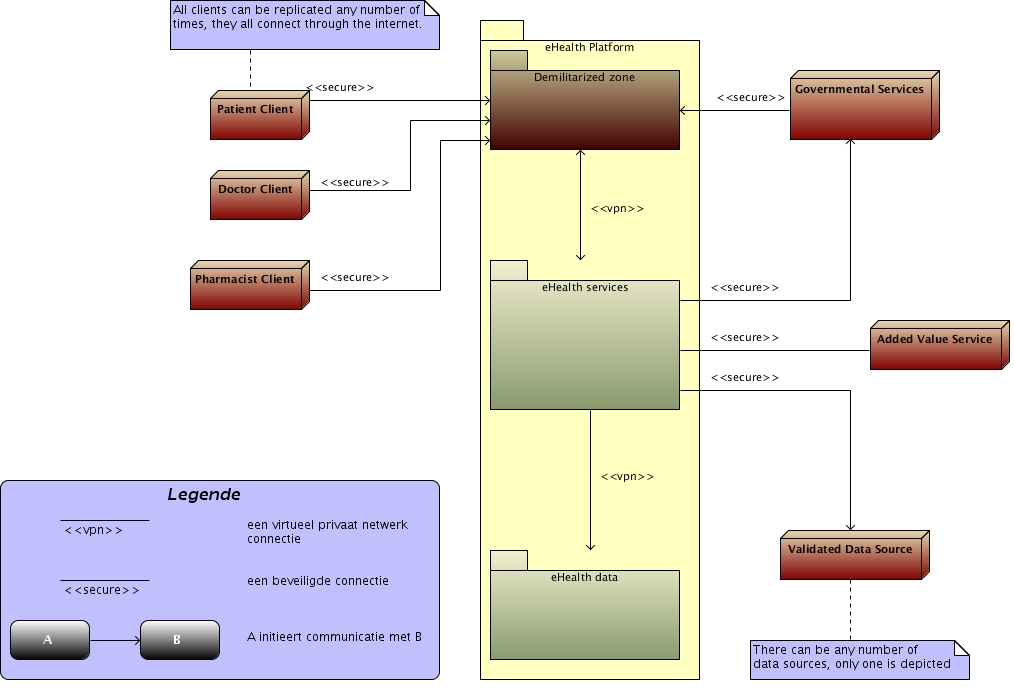
\includegraphics[width=\textwidth]{../images/deployment_DMZ.jpg}
	\caption{deployment diagram giving a high-level overview of the system}
    \end{figure}
 \end{center}

\subsection{Element catalog}

\subsubsection{Elements and their properties}

\begin{enumerate}
\item \textbf{Card Reader}\\*
Een gespecialiseerde hardware node die in staat is om data van een elektronische kaart te lezen en er ook data op te schrijven. Het kan ook data tekenen en encrypteren met behulp van de keys beschikbaar op de kaart aanwezig in de lezer. Meer info hierover vind je in sectie \ref{sec:deployment_clients}.
\item \textbf{Patient Client}\\*
De PC van een patient. Meer info vind je in sectie \ref{sec:deployment_clients}.
\item \textbf{Doctor Client}\\*
De PC van een dokter. Meer info vind je in sectie \ref{sec:deployment_clients}.
\item \textbf{Pharmacist Client}\\*
De PC van een apotheker. Meer info vind je in sectie \ref{sec:deployment_clients}.
\item \textbf{Demilitarized Zone}\\*
Een gedeelte van het eHealth platform waar publieke services zoals web services en de API zullen zitten. Deze zone vereist geen authenticatie noch authorizatie, het is het toegangspunt tot het platform voor externe gebruikers. Een verdere uitwerking van dit element vind je in sectie \ref{sec:deployment_services}.
\item \textbf{eHealth Services}\\*
Gedeelte van het eHealth platform dat alle business logica (services) bevat. Een verdere uitwerking van dit element vind je in sectie \ref{sec:deployment_services}.
\item \textbf{eHealth Data}\\*
Gedeelte van het eHealth platform dat alle data servers bevat. Een verdere uitwerking van dit element vind je in sectie \ref{sec:deployment_data}.
\item \textbf{Validated Data Source}\\*
Een externe node die gevalideerde medische data aanbiedt. Merk op dat hoewel er slechts 1 node getekend staat, er zo een heel scala aan data bronnen bestaan. Het platform moet in staat zijn om verschillende \textit{validated data sources} aan te bieden aan gebruikers. Om dit makkelijk te doen, zal er een interface gedefiniëerd worden die alle aanbieders van deze gegevensbronnen zullen moeten implementeren als ze willen dat de gegevens beschikbaar gesteld worden via het eHealth platform.
\item \textbf{Governmental Services}\\*
Een externe node waarop de overheid allerhande services aanbiedt zoals het RIZIV en ook een service waarmee belangrijke data gelogd kan worden.
\item \textbf{Added Value Service}\\*
Een externe node die extra services aanbied voor gebruikers van het system.
\end{enumerate}

\subsubsection{Relations and their properties}
\label{subsubsec:relations_deployment}
Er zijn drie verschillende soorten connecties te onderscheiden : 
\begin{enumerate}
 \item \textbf{Vertrouwde connecties}\\*
Dit zijn de connecties op het diagram aangeduid met het stereotype 'trusted'. Dit zijn connecties die volledig te vertrouwen zijn. Het gaat hier om de connectie tussen een client node en de kaart lezer. Hier moeten we qua security niet al te veel aandacht aan geven aangezien dit gewoon een rechtstreekse connectie is tussen de kaartlezer en de client node, hier kunnen geen aanvallers aan. 
\item \textbf{Beveiligde connecties}\\*
Dit zijn de connecties op het diagram aangeduid met het stereotype 'secure'. Dit zijn connecties over het internet die goed beveiligd moeten zijn tegen aanvallers. Dit houdt in dat de twee interagerende nodes moeten weten wie de andere is én dat de communicatie geëncrypteerd is, zodat luistervinken geen nuttige data te pakken krijgen.
\item \textbf{Virtueel private netwerk connecties}\\*
Dit zijn de connectie sop het diagram aangeduid met het stereotype 'vpn'. Deze connecties gaan ook over het internet, maar ze maken deel uit van een virtueel privaat netwerk.
\end{enumerate}

\subsubsection{Element interfaces}

De interfaces van de verschillende componenten in de nodes staan beschreven in de secties met de client-server views.

\subsubsection{Element behavior}
[Niet van toepassing]

\clearpage
\subsection{Context diagram}

\begin{center}
    \begin{figure}[!h]
      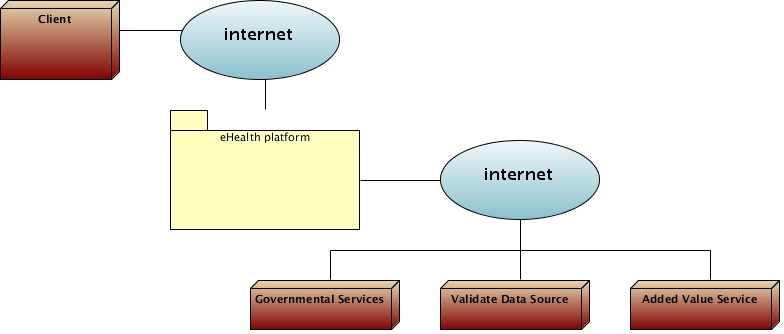
\includegraphics[scale=0.60]{../images/deployment_DMZ_context.jpg}
	\caption{Context diagram for the deployment diagram giving a high-level overview of the system}
    \end{figure}
 \end{center}

\subsection{Variability guide}
[Niet van toepassing]

\subsection{Architecture background}

Het eHealth platform wordt opgedeeld in drie delen. Aan de ene kant hebben we een demilitarized zone (DMZ), aan de andere services en data. Door alle clients te laten connecteren langst de demilitarized zone creëren we een centrale plaats vanwaar alle toegang tot het systeem komt. Dit maakt het makkelijker om het systeem te beveiligen en dus ook makkelijker om te voldoen aan de vereiste dat alle toegang tot het platform geauthoriseerd en beveiligd moet worden. Services en data worden ook van elkaar gescheiden wat resulteert in een grotere modulariteit wat het makkelijker maakt om het geheel te implementeren en te testen.

Om ervoor te zorgen dat de demilitarized zone niet omzeild word door een eventuele aanvaller, wordt er gebruikt gemaakt van virtual private networks (VPNs). Dit bevordert de schaalbaarheid, onderhoudbaarheid en variabiliteit van het systeem aangezien het relatief gemakkelijk is om een nieuwe node toe te voegen moest het nodig zijn. Een VPN wordt ook gebruikt voor alle communicatie tussen de services en data lagen. Een nadeel van de DMZ is dat het een bottleneck vormt voor alle toegang tot het platform. Daarom zullen performantie en beschikbaarheid belangrijke drivers zijn voor de verdere decompositie van de DMZ.

Tenslotte zien we dat de verbinding tussen de eHealth services en de overheid slechts in 1 richting gaat, maar vanuit de overheid kan er wel naar de DMZ gegaan worden. Dit komt doordat de overheid via het internet zal connecteren, waardoor we niet kunnen toelaten dat die alle security maatregelen omzeilt.

\subsection{Other information}
[Niet van toepassing]

\subsection{Related view packets}

De verschillende delen in deze view worden nog verder uitgewerkt in aparte secties. Meer info over de verschillende clients is te vinden in sectie \ref{sec:deployment_clients}. Een uitwerking van de DMZ en de services wordt getoond in sectie \ref{sec:deployment_services} en over de data in het platform vind je meer in sectie \ref{sec:deployment_data}.

\section{Deployment view clients}
\label{sec:deployment_clients}

\subsection{Primary presentation}
\begin{center}
    \begin{figure}[!h]
      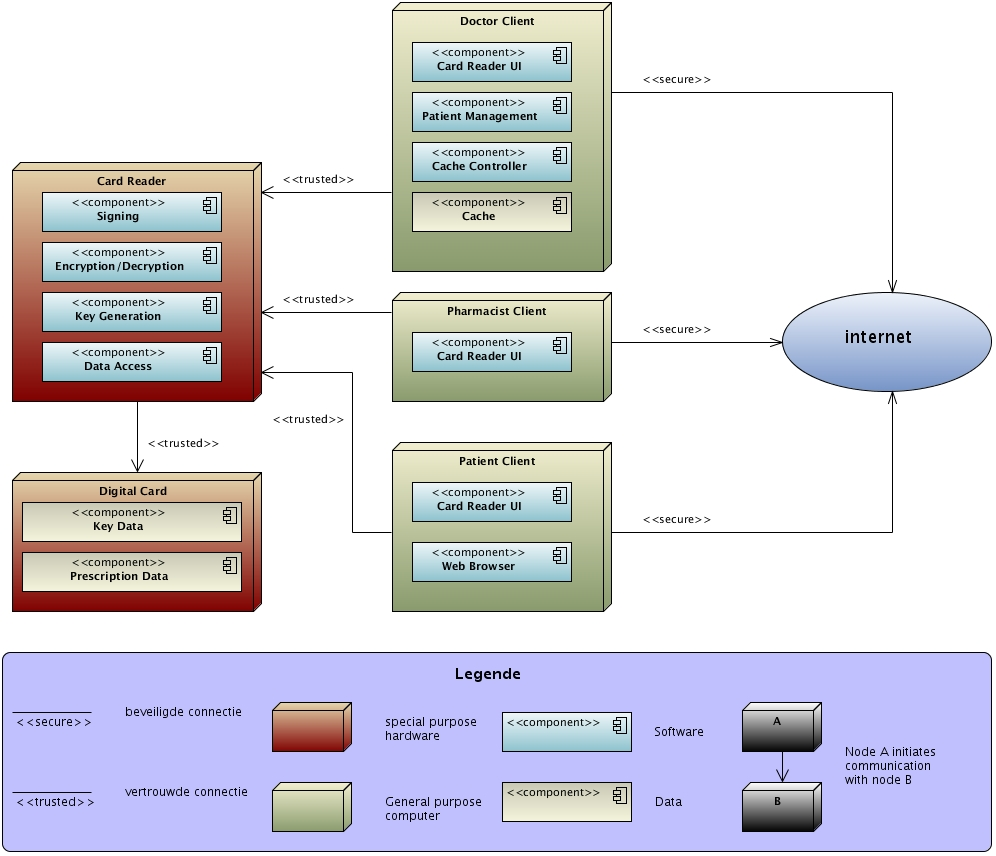
\includegraphics[width=\textwidth]{../images/deployment_clients.jpg}
	\caption{Deployment diagram focused on the various clients in the system}
    \end{figure}
  \end{center}

\subsection{Element catalog}

\subsubsection{Elements and their properties}

\begin{enumerate}
 \item \textbf{Digital Card}\\
Deze node stelt een digitale kaart voor die elke patient en dokter toegewezen krijgt van de overheid. Deze node zal geen echte software bevatten, maar dient enkel als data opslag. Volgende twee soorten data kunnen we onderscheiden :
\begin{enumerate}
 \item \textbf{Key Data}\\*
De keys op de kaart. Elke kaart zal een publieke en private sleutel bevatten waarmee getekend en/of geëncrypteerd kan worden met behulp van de elektronische kaartlezer.
\item \textbf{Prescription Data}\\*
De voorschriften die een dokter voorschrijft voor een patient zullen op de kaart bijgehouden worden, zodat deze terug uitgelezen kunnen worden bij het ophalen/bestellen van medicatie bij de apotheker/e-pharmacy.
\end{enumerate}

\item \textbf{Card Reader}\\*
De elektronische kaartlezer bevat volgende software componenten : 
\begin{enumerate}
\item \textbf{Signing}\\*
Software verantwoordelijk voor het tekenen van documenten (voorschriften).
\item \textbf{Encryption/Decryption}\\*
Deze component kan data versleutelen en terug ontcijferen met behulp van de keys die op de kaart staan die in de kaartlezer zit.
\item \textbf{Key Generation}\\*
Sleutels kunnen ook gegenereerd worden. Dit zal ondermeer gebruikt worden voor het tijdelijk toekennen van toegang tot het globaal medisch dossier.
\item \textbf{Data Access}\\*
Deze component is verantwoordelijk voor het ophalen en schrijven van data van/op de elektronische kaart.
\end{enumerate}

\item \textbf{Doctor Client}\\*
Stelt een node voor gebruikt door een dokter. Dit kan eender welke soort van node zijn (PC, PDA, laptop, ...). De node bestaat uit volgende componenten : 
\begin{enumerate}
 \item \textbf{Card Reader UI}\\*
De user interface die toegang biedt tot alle functionaliteit van de elektronische kaartlezer.
\item \textbf{Patient Management}\\*
Deze software staat in voor het beheer van het klantenbestand van de dokter.
\item \textbf{Cache Controller}\\*
Component die het ophalen en wegschrijven van patiënt data in zijn/haar globaal medisch dossier controleert. Een meer gedetailleerde uitleg kan gevonden worden in sectie \ref{Client and Server View: Client}.
\item \textbf{Cache}\\*
In de nodes die dokters gebruiken wordt een cache gebruikt met globaal medische dossiers van patiënten van de dokter. Het lezen en schrijven van deze cache wordt beheert door de \textit{Cache Controller}.
\end{enumerate}

\item \textbf{Patient Client}\\*
Deze node is de tool van de patient. Het is gewoon een ordinaire computer, laptop of PDA. De enige custom software die deze node nodig heeft is software die de node in staat stelt om te communiceren met de elektronische kaartlezer. Voor de rest kan een patiënt alle nodige activiteiten doen met behulp van een normale web browser, die wel in staat moet zijn om met geëncrypteerde verbindingen om te gaan.

\item \textbf{Pharmacist Client}\\*
Node voor een apotheker. Weer is de enige custom software nodig, software om te communiceren met de kaartlezer, alle andere activiteiten kunnen met een gewone web browser uitgevoerd worden.

\end{enumerate}


\subsubsection{Relations and their properties}

Zie sectie \ref{subsubsec:relations_deployment}.

\subsubsection{Element interfaces}

[Niet van toepassing]

\subsubsection{Element behavior}

Zie sectie \ref{Client and Server View: Client}.

\subsection{Context diagram}

\begin{center}
    \begin{figure}[!h]
      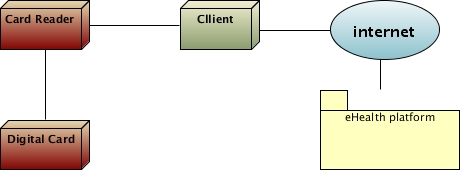
\includegraphics[width=\textwidth]{../images/deployment_clients_context.jpg}
	\caption{Context diagram for de deployment view focused on the clients}
    \end{figure}
  \end{center}

\subsection{Variability guide}
Zie sectie \ref{Client and Server View: Client}.

\subsection{Architecture background}
Een dokter moet in staat zijn om ten alle tijden de globaal medische dossiers van zijn patiënten in te kijken, ook wanneer hij geen actieve internetverbinding heeft en dus niet met het eHealth platform kan communiceren. Daarom is het belangrijk dat een dokter een lokale cache heeft. Meer informatie over de werking van deze cache vind je in sectie \ref{Client and Server View: Client}.
Ook één van de vereisten is dat voorschriften aangemaakt en gevalideerd kunnen worden binnen de 3 seconden , verder moeten voorschriften ook door een dokter aangemaakt kunnen worden, zelfs in geval van een gedeeltelijke systeem of netwerk faling. Daarom zorgen we ervoor dat voorschriften op de elektronische kaart van de patient gezet zullen worden. De dokter kan dan ook wanneer hij offline is het voorschrift creëren (de registratie van het voorschrift in het GMR van de patient wordt dan gequeued tot de dokter terug online is) en de apotheker is in staat om het voorschrift te valideren, ook wanneer die offline is. Doordat dit enkel lokale bewerkingen inhoudt, is de 3 seconden vereiste zeker haalbaar.

\subsection{Other information}
[Niet van toepassing]

\subsection{Related view packets}
Via het internet maken alle clients verbinding met het eHealth platform, dit gedeelte van het systeem vind je gedetailleerder terug in sectie \ref{sec:deployment_services}.

\clearpage
\section{Deployment view services}
\label{sec:deployment_services}

\subsection{Primary presentation}
\begin{center}
    \begin{figure}[!h]
      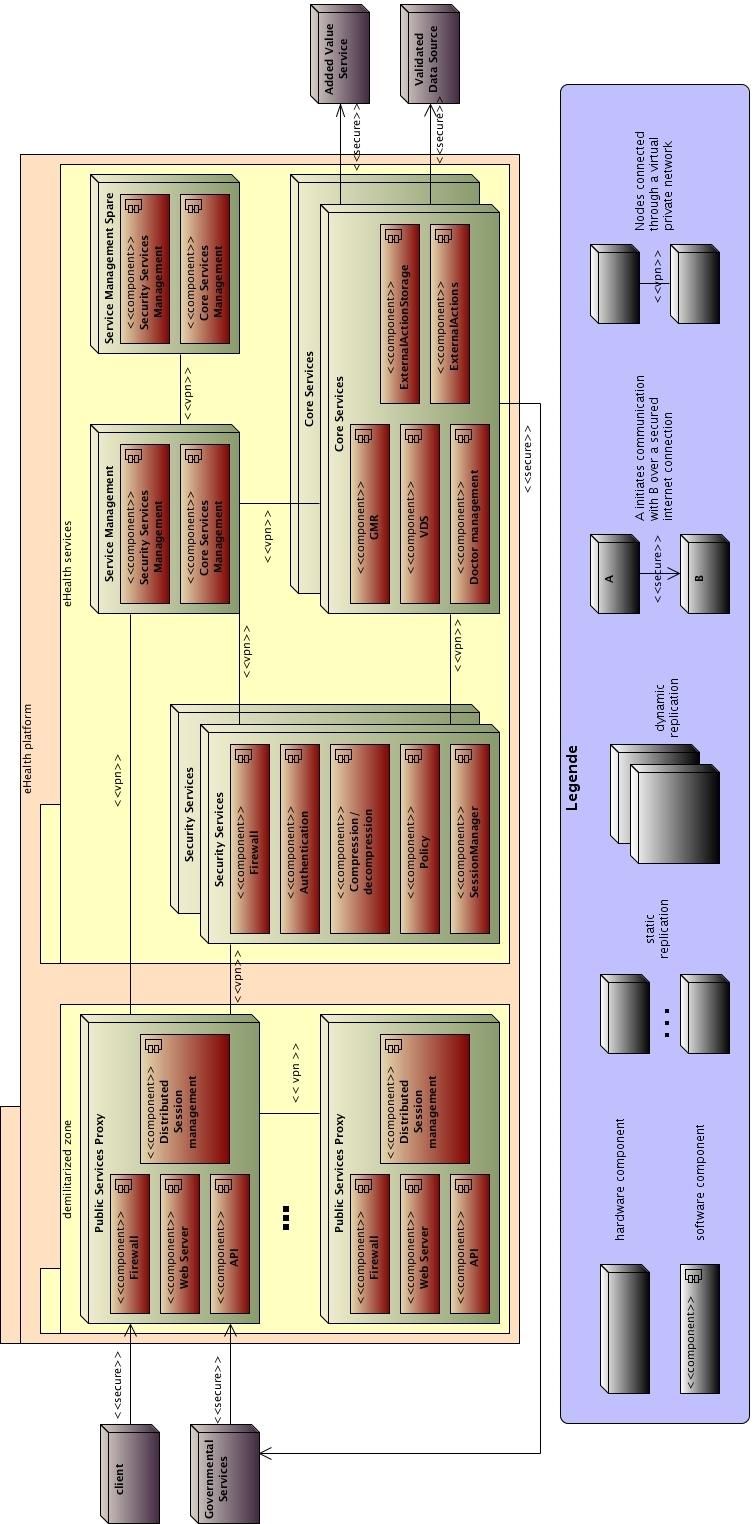
\includegraphics[width=\textwidth]{../images/deployment_services.jpg}
	\caption{Deployment diagram focused on the services in the platform}
    \end{figure}
  \end{center}

\subsection{Element catalog}

\subsubsection{Elements and their properties}
\begin{enumerate}
 \item \textbf{Client}\\*
Stelt de client nodes voor zoals getoond in sectie \ref{sec:deployment_clients}. Hoewel er maar 1 node getoond is, zijn er in de praktijk zeer veel verschillende clients.
\item \textbf{Governmental Server}\\*
Server die de nodige services van de overheid voorziet.
\item \textbf{Validated Data Source}\\*
Stelt de \textit{validate data sources} voor, in de praktijk zijn er meerdere \textit{validated data sources} hoewel er op het diagram slechts 1 getoond wordt.
\item \textbf{Added Value Service}\\*
Stelt de \textit{added value services} voor, weer zullen dit er meerdere zijn.
\item \textbf{Public Services Proxy}\\*
Deze node doet dienst als proxy, zoals z'n naam doet vermoeden. Meer specifiek is het een \textit{reverse proxy}. Deze wordt ingezet om de belasting vanuit het internet naar de security services nodes gelijkmatiger te verdelen, zowel om beveiligings als om \textit{loadbalancing} redenen. Buiten dat, bevat deze node ook een web server en biedt die de API aan aan externe \textit{added value services}. Deze nodes worden statisch gerepliceerd. De public services proxy bevat volgende software componenten : 
\begin{enumerate}
 \item \textbf{Firewall}\\*
 Deze firewall is de eerste verdedigings linie voor het platform en dient het verkeer naar de DMZ toe te filteren zodat enkel connecties specifiek naar de DMZ doorgelaten worden.
\item \textbf{Web Server}\\*
De web server biedt de publieke web services van het systeem aan. Indien dit om zeer algemene data gaat, dient het verkeer niet verder te komen dan de DMZ. Is er echter medische data nodig, dan zal de web server requests doorsturen naar de services laag in het platform.
\item \textbf{API}\\*
Er moet een API voorzien worden voor externe services die gebruik willen maken van het platform. Deze component voorziet deze API en zal alle calls doorsturen naar de services laag van het platform.
\item \textbf{Distributed Session Management}\\*
Het is ongewenst dat een gebruiker zich voor elke actie die hij/zij wil ondernemen terug opnieuw moet inloggen. Er zullen dus sessies bijgehouden moeten worden. Het is niet zo veilig dit te doen binnen de DMZ, dus de authenticatie sessie - data zal bijgehouden worden in de \textit{security services} nodes in de services laag (zie bij security services hier onder). Er zullen meerdere \textit{security services} nodes zijn, dus zal het verkeer van een bepaalde gebruiker gedurende de hele sessie langst dezelfde \textit{security services} node moeten gaan. Het kan zijn, door de structuur en werking van het internet, dat gedurende dezelfde sessie niet dezelfde proxy gebruikt wordt. Om dus toch te kunnen garanderen dat voor één bepaalde sessie steeds dezelfde \textit{security services} node gebruikt wordt, wordt deze component geïntroduceerd. Het enige wat die moet doen is bijhouden welke sessie bij welke \textit{security services} node hoort en dit ook doorgeven aan de andere actieve \textit{Public Services Proxies}.
\end{enumerate}

\item \textbf{Security Services}\\*
Deze node vomt de tweede lijn van verdediging voor het platform. Alle verkeer die de core services van het platform wil gebruiken zal langst hier moeten. Het zorgt ervoor dat enkel geauthenticeerde requests met de juiste authorisatie toegelaten worden. Deze node zal dynamisch gerepliceerd worden, later wordt hier wat verder op in gegaan. Volgende software componenten worden op deze node geplaatst : 
\begin{enumerate}
 \item \textbf{Firewall}\\*
Deze firewall zal ervoor zorgen dat enkel connecties vanuit de DMZ toegelaten worden binnen de services laag van het eHealth platform.
\item \textbf{Authentication}\\*
Component die de authenticatie van gebruikers zal afhandelen. Zie sectie \ref{Client and Server View: Security} voor meer informatie.
\item \textbf{Compession/Decomporession}\\*
Component die de compressie en decompressie van data zal afhandelen. Weer biedt sectie \ref{Client and Server View: Security} meer gedetailleerde informatie.
\item \textbf{Policy}\\*
Deze component zal verantwoordelijk zijn voor zowel de authorisatie van requests, als ook voor het beheren van access policies, zoals het geven van toestemming aan dokters om het globaal medisch dossier van een patient in te kijken. Sectie \ref{Client and Server View: Server} legt dit verder uit.
\item \textbf{SessionManager}\\*
We willen niet dat een gebruiker zich voor elke nieuwe request opnieuw moet inloggen. We zullen dus sessie data nodig hebben. Deze component zal het beheer van die sessie data controleren.
\end{enumerate}

\item \textbf{Core Services}\\*
Deze node bundelt alle kern services samen die nodig zijn voor de werking van het eHealth platform. Volgende componenten in deze node stellen al die services voor : 
\begin{enumerate}
 \item \textbf{GMR}\\*
Component die alle functionaliteit aanbiedt voor het lezen, schrijven en aanpassen van data in globaal medische dossiers.
\item \textbf{Doctor Management}\\*
Beheert alle data gerelateerd met dokters. Registratie van dokters en de registratie van patiënten van dokters gebeurt aan de hand van deze component.
\item \textbf{VDS}\\*
Dit stuk software zal alle functionaliteit aanbieden om data te kunnen ophalen van de \textit{validated data sources}, alsook functionaliteit voor het toevoegen van validated data sources aan het systeem. Wanneer zo'n gegevensbron toegevoegd dient te worden, zal die gegevensbron aangeboden moeten worden met een interface die vastgelegd wordt door ons systeem. 
\item \textbf{ExternalActions}\\*
Component die de link met de \textit{Governmental Services} voorziet (loggen en RIZIV).
\item \textbf{ExternalActionsStorage}\\*
Indien het RIZIV of de log-functionaliteit van de overheid tijdelijk niet beschikbaar zijn, zullen alle requests naar de ExternalActions component tijdelijk bijgehouden worden in deze component in twee FIFO-queues, één voor elke dienst. Wanneer de diensten terug online komen, zullen de queues verwerkt worden waardoor de nodige data naar de diensten verstuurd kan worden.
\end{enumerate}

\item \textbf{Service Management \textit{(Spare)}}\\*
Deze node zal verantwoordelijk zijn voor het beheren van de verschillende services in het systeem. Zoals je kan zien op het diagram worden de security services en de core services beiden apart dynamisch gerepliceerd. Dit houdt in dat het aantal actieve processen gedediceerd voor deze twee onderdelen afhankelijk zal zijn van de belasting van het systeem. Deze node controleert dit alles. Het bevat twee aparte componenten, 1 voor de security services en 1 voor de core services. De node zal ook verantwoordelijk zijn voor het registreren en het deregistreren van de verschillende security services processen aan de \textit{Public Services Proxies} zodat deze weten welke er beschikbaar zijn.

\end{enumerate}


\subsubsection{Relations and their properties}
Zie sectie \ref{subsubsec:relations_deployment} voor meer info over de verschillende connecties tussen de nodes.

\subsubsection{Element interfaces}
[Niet van toepassing]

\subsubsection{Element behavior}
Wanneer een request gemaakt wordt naar het platform, zal deze via de \textit{Public Services Proxy} moeten. Deze zal moeten beslissen naar welke van de actieve \textit{Security Services} servers de request doorgestuurd zal worden. Zoals eerder vermeld zal dit voor een bepaalde sessie steeds dezelfde moeten zijn om authenticatie bij te kunnen houden. Dus als de \textit{Public Services Proxy} een request krijgt van een sessie die reeds in het \textit{Distributed Session Management} geregistreerd staat, moet er geen keuze gemaakt worden. Wanneer een request binnenkomt die nog niet geregistreerd is, zal de \textit{Public Services Proxy} een korte ping-boodschap sturen naar de 3 \textit{Security Services} servers die het minst in het \textit{Distributed Session Management} gekoppeld zijn aan een sessie. De eerste die hierop antwoord zal dan gekozen worden om de request naar door te sturen.

De \textit{Public Services Proxy} moet natuurlijk ook weten welke \textit{Security Services} servers er beschikbaar zijn. Hiervoor is de \textit{Service Management} server verantwoordelijk. Deze zal aan de hand van een ping-echo techniek elk van de \textit{Security Services} servers controleren. Wanneer 1 van die servers niet meer antwoord, betekent dit dat die node faalt en zal dit doorgegeven worden aan de \textit{Public Services Proxies}. In de ping-echo boodschap zullen de \textit{Security Services} servers ook hun huidige load aangeven. Wanneer de \textit{Service Management} server merkt dat alle servers zwaar geladen zijn.zal deze beslissen om een nieuwe op te starten. Dit zal dan ook doorgegeven worden aan de \textit{Public Services Proxies}.

Dit zelfde systeem wordt gebruikt voor de connectie tussen de \textit{Security Services} servers en de \textit{Core Services} servers. Een \textit{Security Services} zal eerst naar 3 verschillende \textit{Core Services} servers een korte ping-boodschap sturen en vervolgens diegene die het snelst antwoord kiezen om verder mee te werken. De \textit{Service Management} server zal er nu ook weer voor zorgen dat de \textit{Security Services} servers weten met welke \textit{Core Services} servers ze kunnen connecteren en deze laatste ook monitoren en dynamisch toevoegen indien nodig.

\subsection{Context diagram}
\begin{center}
    \begin{figure}[!h]
      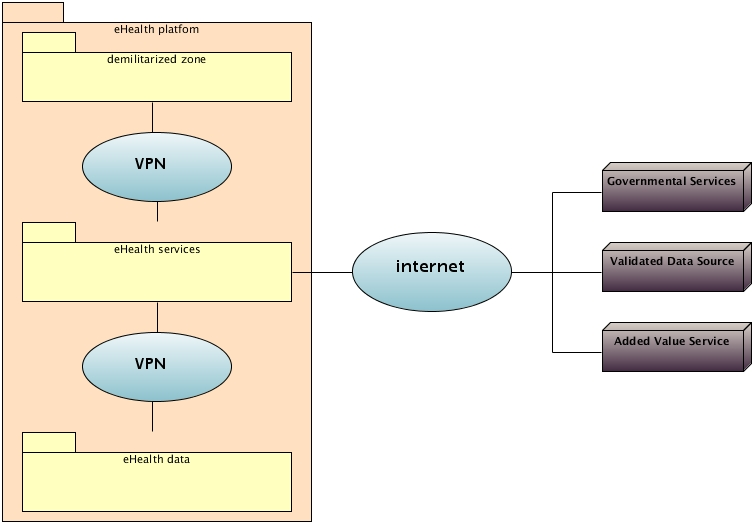
\includegraphics[scale=0.50, width=\textwidth]{../images/deployment_services_context.jpg}
	\caption{Context diagram for the deployment diagram focused on the services in the platform}
    \end{figure}
  \end{center}

\subsection{Variability guide}
[Niet van toepassing]

\subsection{Architecture background}
\label{subsec:arch_back_dep_serv}
Omwille van de zware beschikbaarheids vereisten - maximum 2 minuten downtime per jaar - hebben we alle nodes gedupliceerd, zodat er zeker niet één \textit{single point of failure} in het systeem zit. In het gedeelte bescreven in deze sectie worden 3 verschillende replicatie-technieken gebruikt. De \textit{Public Services Proxy} servers worden statisch gerepliceerd. Dit betekent dat het aantal servers niet door het systeem zelf zal gewijzigd worden. Natuurlijk kunnen er wel manueel nieuwe servers toegevoegd worden.

De replicatie-techniek gebruikt voor voor de \textit{Security Management} servers is een \textit{spare}. De gewone server zal er tijdens het lopen voor zorgen dat de staat van de reserve steeds in real-time mee ge-update wordt. Dit zal gebeuren op een regelmatig (kort) interval. Wanneer de reserve een aantal van die updates mist, neemt deze aan dat de primaire \textit{Security Management} server gefaald heeft en zal die voortaan de functies van de primaire overnemen.

Ten slotte wordt er ook gebruik gemaakt van dynamische replicatie voor zowel de \textit{Security Services} als de \textit{Core Services}. Dit zorgt voor een goede schaalbaarheid van het systeem aangezien het systeem zich zal aanpassen aan de load.

Performantie is natuurlijk ook belangrijk. Bepaalde gegevens moeten binnen bepaalde tijdspannes beschikbaar zijn. Daarom gebruiken we de methode hierboven beschreven om van de \textit{Public Services Proxies} naar de \textit{Security Services} en van de \textit{Security Services} naar de \textit{Core Services} te gaan. We zullen telkens eerst een korte ping-boodschap sturen naar minstens 3 nodes en op basis van de antwoorden op deze ping een keuze maken. Dit doen we om ervoor te zorgen dat we niet te veel tijd verspillen met het wachten op een timeout met een falende component. Ook is dit een primitieve vorm van dynamisch loadbalancing, het antwoord dat het eerst terugkomt zal gewoon de snelste (en dus waarschijnlijk minst belaste) route volgen.

\subsection{Other information}

Het aantal \textit{Public Services Proxies} moet nog bepaald worden. Hiervoor zal eerst onderzoek gedaan moeten worden naar de verwachte load van het systeem en moeten we weten welke systemen we beschikbaar hebben.

\subsection{Related view packets}
Voor meer uitleg over het data gedeelte verbonden met dit service gedeelte, zie sectie \ref{sec:deployment_data}.\\*
Sectie \ref{Client and Server View: Server} geeft wat meer info over de verschillende componenten besproken in dit view.

\clearpage
\section{Deployment view data}
\label{sec:deployment_data}

\subsection{Primary presentation}
\begin{center}
    \begin{figure}[!h]
      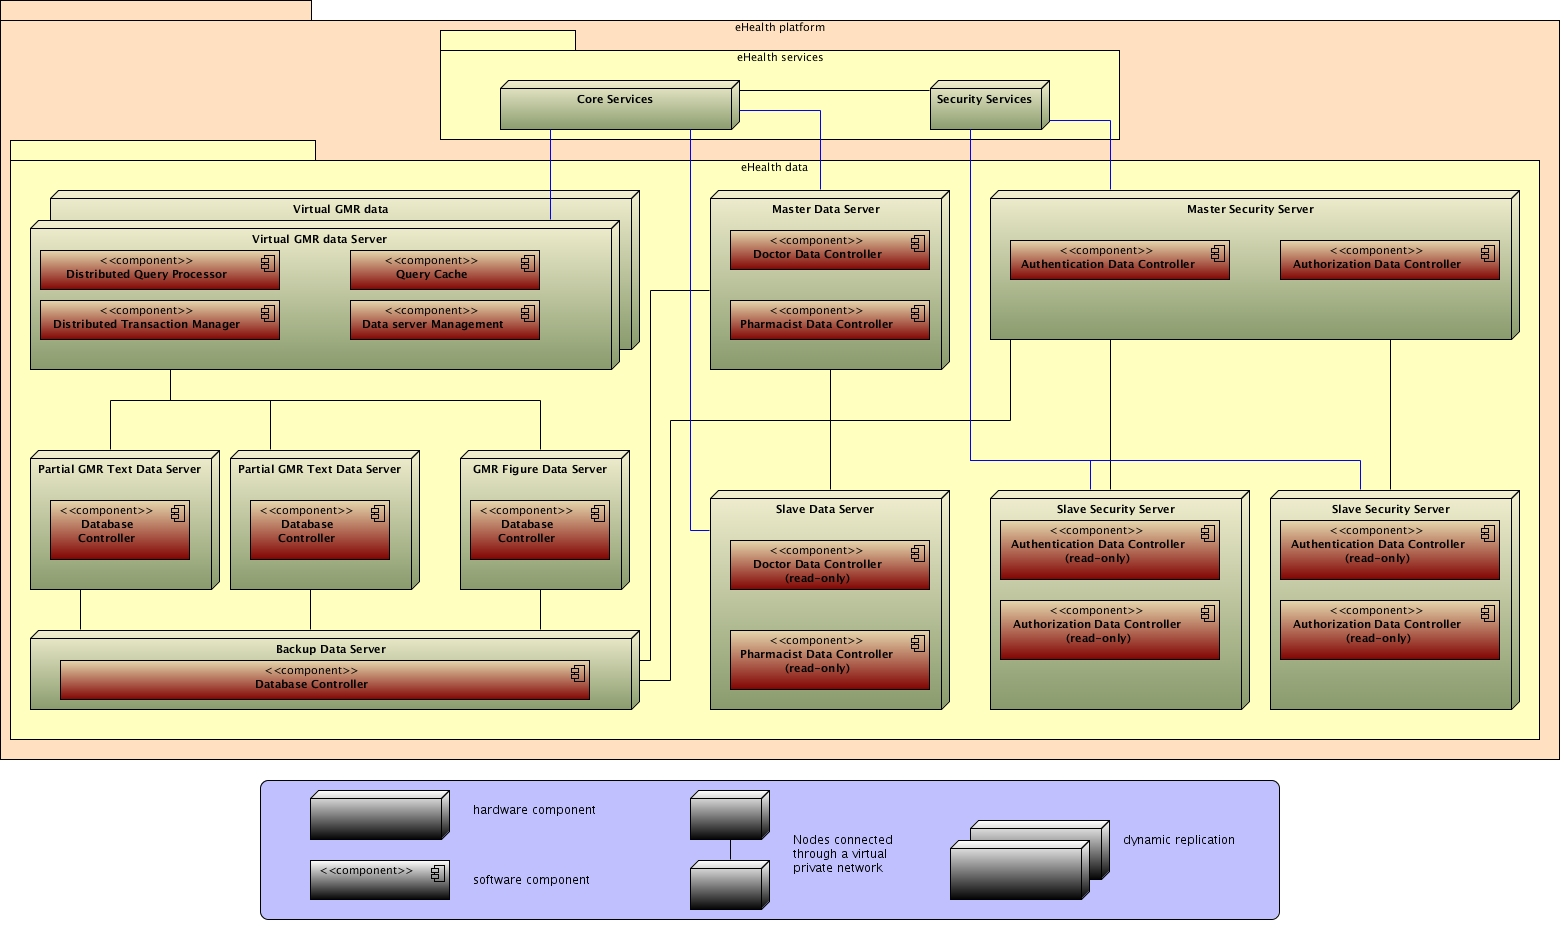
\includegraphics[width=\textwidth]{../images/deployment_data.jpg}
	\caption{Deployment diagram focused on the data storage in the platform}
    \end{figure}
  \end{center}

\subsection{Element catalog}

\subsubsection{Elements and their properties}
\begin{enumerate}
 \item \textbf{Core Services}\\*
Node die alle kern services van het systeem bundelt. Meer info vind je in sectie \ref{sec:deployment_services}.
\item \textbf{Security Service}\\*
Node die alle security services van het systeem bundelt. Meer info vind je in sectie \ref{sec:deployment_services}.
\item \textbf{Virtual GMR Data Server}\\*
Deze server zal alle GMR data als een coherent geheel beschikbaar stellen. Aangezien volgens de wetgeving niet alle data van één enkel GMR op 1 plaats opgeslagen mag worden, hebben we deze node nodig die de nodige delen van een opgevraagd GMR zal ophalen op de aparte data servers. Deze node zal dynamisch gerepliceerd worden volgens de load, net zoals de \textit{Security Services} en de \textit{Core Services} in de services laag. Volgende componenten zitten in deze node : 
\begin{enumerate}
 \item \textbf{Distributed Query Processor}\\*
Deze component zal ervoor zorgen dat queries voor GMR data correct opgesplitst zullen worden in aparte queries voor de aparte data servers. Het laat die aparte queries hun werk doen en zal achteraf alle verkregen dat terug bijeenzetten tot een geheel dat dan als antwoord dient op de orginele query.
\item \textbf{Distributed Transaction Manager}\\*
Dit stuk software is verantwoordelijk voor de consistentie van de GMR data. Wanneer er een query uitgevoerd moet worden die gegevens update of wegschrijft, zal deze component er verantwoordelijk voor zijn dat alle subqueries uitgevoerd worden. Indien er 1 van de subqueries faalt, zullen de andere subqueries ongedaan gemaakt worden door dit element.
\item \textbf{Query Cache}\\*
Dit element zal tijdelijk de laatste queries die uitgevoerd zijn op de GMR data bijhouden, dit zal nodig zijn voor eventuele herstellingsoperaties bij het falen van 1 van de data servers zoals uitgelegd in sectie \ref{subsubsec:dep_data_behavior}.
\item \textbf{Data Server Management}\\*
Dit element biedt functionaliteit om de aparte data servers te beheren.
\item \textbf{Indexation}\\*
Deze component stelt de opslag voor van een indexatie van de data server zodat gemakkelijk teruggevonden kan worden waar het GMR van een bepaalde patiënt gevonden kan worden.
\end{enumerate}

\item \textbf{Partial GMR Text Data Server}\\*
Deze server zal tekstuele GMR data bevatten. Het zal niet alle data van 1 GMR bevatten, maar slechts gedeeltes van die date, aangezien dit bij wet voorgeschreven wordt. Deze servers zullen statisch gerepliceerd worden. De node bevat volgende software componenten : 
\begin{enumerate}
 \item \textbf{Encryption/Decryption}\\*
Alle data op deze node dient geëncypteerd opgeslagen worden.Deze component zorgt daarvoor en zorgt er ook voor dat wanneer er data opgevraagd wordt, deze data ontcijferd wordt.
\item \textbf{DB Controller}\\*
Algemene database controller die de eigenlijke data access verzorgt.
\end{enumerate}

\item \textbf{GMR Figure Data Server}\\*
Net hetzelfde als de \textit{Partial GMR Text Data Server}, behalve het soort van data dat erin opgeslagen wordt is anders.

\item \textbf{Backup Data Server}\\*
Deze servers zijn backups van de data servers waarmee ze verbonden zijn.

\item \textbf{Master Data Server}\\*
\label{masdatserv}
Deze node zal data bijhouden die geen deel is van GMR data, namelijk data over dokters en welke patienten bij welke dokter horen. Deze node is statisch gerepliceerd door middel van een master-slave communicatie. Deze node is de master, wat wil zeggen dat op deze node geschreven en gelezen kan worden. De andere nodes zijn slaves, wat wil zeggen dat daar enkel van gelezen kan worden. Merk op dat hoewel er maar 1 slave node getoond wordt, er meerdere mogelijk zijn. Deze nodes hebben, net zoals de \textit{Partial GMR Text Data Servers}, hun eigen private sleutel waarmee alle data op die node geëncrypteerd en gedecrypteerd kan worden.
\item \textbf{Slave Data Server}\\*
Zie item \ref{masdatserv}.

\item \textbf{Master Security Server}\\*
\label{massecserv}
Deze node zal alle security gerelateerde data bijhouden (authenticatie en authorisatie data). Ook deze node wordt gerepliceerd door middel van een master-slave configuratie en wordt beveiligd door een eigen private sleutel om data mee te versleutelen, net zoals bij de \textit{Master Data Server}.
\item \textbf{Slave Security Server}\\*
zie item \ref{massecserv}.


\end{enumerate}

\subsubsection{Relations and their properties}
Zie sectie \ref{subsubsec:relations_deployment} voor een uitleg over de types van connecties.

\subsubsection{Element interfaces}
[Niet van toepassing]

\subsubsection{Element behavior}
\label{subsubsec:dep_data_behavior}
Als er vanuit de \textit{Core Services} data opgevraagd moet worden, zal weer hetzelfde mechanisme in werking treden als bij de communicatie tussen de \textit{Public Services Proxies} en de \textit{Security Services} beschreven in sectie \ref{subsec:arch_back_dep_serv}. Er zal eerst een ping bericht gestuurd worden naar minstens 3 virtuele servers en diegene die het snelst antwoord zal gekozen worden om verder mee te werken.

Wanneer een virtuele data server een query krijgt voor GMR data, zal deze die query opsplitsen in subqueries die de verschillende delen van de data zal ophalen van de verschillende data servers die elk partiële data bevatten. Daarna worden die subqueries uitgevoerd op de correcte data server en de resultaten worden samengegoten tot 1 geheel dat als antwoord dient voor de originele query. Elke query zal door de virtuele data server ook gecached worden. Indien de query data update of toevoegt, zal de \textit{Distributed Session Manager} ervoor zorgen dat de volledige operatie uitgevoerd wordt, of indien dit niet lukt, de query helemaal geen invloed gehad heeft op de data. Het teruggeven van deze data gebeurt ook in twee delen. Eerst zal alle tekstuele data teruggegeven worden en pas daarna eventuele figuren.

Alle data servers hebben hun eigen private sleutel. Wanneer data toegevoegd wordt, zal die data met die sleutel geëncrypteerd worden vooraleer die opgeslagen wordt. Wanneer er dan data opgevraagd wordt, zal met diezelfde sleutel de data gedecrypteerd worden. Deze data mag echter niet ongeëncrypteerd verstuurd worden, dus moet elke request voor data een andere sleutel meegeven waarmee de data eerst geëncrypteerd zal worden alvorens die doorgestuurd wordt.

De GMR data servers hebben elk een backup data server. Op geregelde tijdstippen worden die backups gesynchroniseerd met de data op de servers. Dit wordt geregeld door de \textit{DB Controller} component. Indien 1 van deze GMR data servers zou falen, dan zal de backup-server dit merken doordat er geen synchronisaties meer plaatsvinden. Indien dit het geval is, spreekt de backup de virtuele data servers aan en vraagt alle relevante queries op die uitgevoerd zijn sinds de laatste synchronisatie van de backup. De backup update zijn gegevens en zal vanaf dan dienst doen als GMR data server.

\clearpage
\subsection{Context diagram}
\begin{center}
    \begin{figure}[!h]
      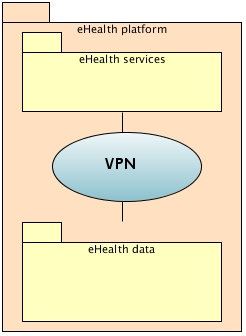
\includegraphics[scale=0.50]{../images/deployment_data_context.jpg}
	\caption{Context diagram for the deployment diagram focused on the data storage in the platform}
    \end{figure}
  \end{center}

\subsection{Variability guide}
Op het diagram, wordt 1 GMR nu opgedeeld in drie stukken : 2 tekstuele stukken en 1 stuk voor andere data (zoals bijv. figuren). Dit kan eventueel nog gewijzigd worden, afhankelijk van de exacte wettelijke voorschriften over de scheiden van de data. Het functioneren van het systeem zal hierdoor niet wijzigen.

Het juiste aantal nodes voor de statisch gerepliceerde servers zal nog bepaald moeten worden aan de hand van een analyse van de verwachte load en de beschikbare communicatie-lijnen en servers. Belangrijk is dat het systeem om moet kunnen met eender welk aantal zodat deze beslissingen later nog aangepast kunnen worden.

\subsection{Architecture background}
Het is bij wet verplicht om de data voor een bepaald GMR verspreid bij te houden, vandaar dat het mechanisme met de virtuele data servers in het systeem geplaatst wordt. Door een data server management component te voorzien in de virtuele data servers, wordt het mogelijk om het aantal servers uit te breiden indien dit nodig moest zijn, wat de variabiliteit van het systeem bevordert. Het verspreiden van de data is ook zeer gunstig vanuit een security standpunt. Moest het zijn dat een aanvaller de disk op 1 van de servers kan kopiëren, zal deze nog steeds niet zijn met de data die hij ervan af gehaald heeft. Ook wordt de data geëncrypteerd, wat de data nog nuttelozer maakt voor een aanvaller.

Om aan de beschikbaarheids-vereisten te voldoen, wordt er gebruik gemaakt van replicatie. Voor de doktor data en de security data wordt dit gedaan aan de hand van een master-slave configuratie. Hierdoor wordt de load van het systeem verspreid over de master en de verschillende slaves om zo ook aan de performantie-vereisten te kunnen voldoen. Aangezien er slechts 1 master is, zou dit een bottleneck kunnen zijn, maar aangezien de doktor en security data waarschijnlijk niet vaak aangepast zullen worden, zal dit geen problemen geven.

Voor de GMR data zou dit wel een performantie bottleneck zijn aangezien deze data veel frequenter aangepast wordt. Daarom voorzien we hier een ander mechanisme. De partiële data servers worden statisch gerepliceerd, zonder hier een master in aan te duiden, er mag naar alle replica's geschreven worden. Wanneer deze servers met elkaar synchroniseren, zal er bij conflicten een merging-techniek gebruikt worden zoals beschreven in sectie \ref{Client and Server View: Server}. Indien het mergen niet lukt, zal 1 van de updates op alle replica's doorgevoerd worden en de andere zal ongedaan gemaakt worden en falen. We kunnen zo'n merging techniek gebruiken aangezien het zeer onwaarschijnlijk is dat dezelfde data op dezelfde moment aangepast wordt.

De performantie-vereisten voor het ophalen van tekstuele data en andere data verschillen nogal wat. Om ervoor te zorgen dat het ophalen van tekst nooit moet wachten op het ophalen van figuren, worden tekst en figuren volledig van elkaar gescheiden. Aangezien tekstuele data striktere performantie-vereisten heeft, geven we telkens eerst de tekstuele data terug en daarna de figuren. Het zoeken naar de locatie van de data zelf mag ook niet langer duren dan 3 seconden. Daarom wordt op de virtuele data servers een index bijgehouden die telkens wanneer nieuwe data toegevoegd wordt ook ge-update zal worden.

\subsection{Other information}
[Niet van toepassing]

\subsection{Related view packets}
Een gedetailleerder zicht op de services verbonden met deze data laag vind je in sectie \ref{sec:deployment_services}.

\clearpage
\section{Interaction Diagrams}
\label{interaction:main}
De sequentiediagrammen geven enkele concrete scenario's die de onderlinge werking van de componenten in het systeem illustreren. Zo wordt getoond hoe een dossier wordt weergegeven en gewijzigd, hoe toegangsrechten worden gegeven op het dossier en hoe voorschriften worden aangemaakt en gevalideerd. Hier wordt de concerete opeenvolging van boodschappen weergegeven die zo een scenario bevat.\\

Bij de communicatie tussen de user applicaties en het e-health platform wordt de verzonden informatie steeds ge-encrypteerd en gecompresseerd. Dit wordt in de diagramma's weggelaten om het overzichtelijker te maken. 


\subsection{Grant access}
\label{interaction:grantAccess}
Wanneer een patient een dokter toegang tot zijn dossier wil geven, voert deze eerst zijn persoonlijke code in om zijn persoonlijke key aan het systeem van de dokter te koppelen. Vanuit de applicatie van de dokter (we veronderstellen hier dat het toegang geven gebeurt bij de eerste consultatie, en niet thuis op voorhand) wordt dan de vraag om de toegangsrechten te wijzigen verstuurd. Ook de persoonlijke toegangscode van de patient wordt gevraagd en nagegaan om te zien of deze de rechten heeft om toegang te verlenen. Wanneer dit in orde is, worden de toegangsrechten tot het dossier zo aangepast dat de dokter er toegang tot heeft voor de periode die patient heeft opgegeven (kan ook permanent zijn). 

\begin{figure}[!h]
  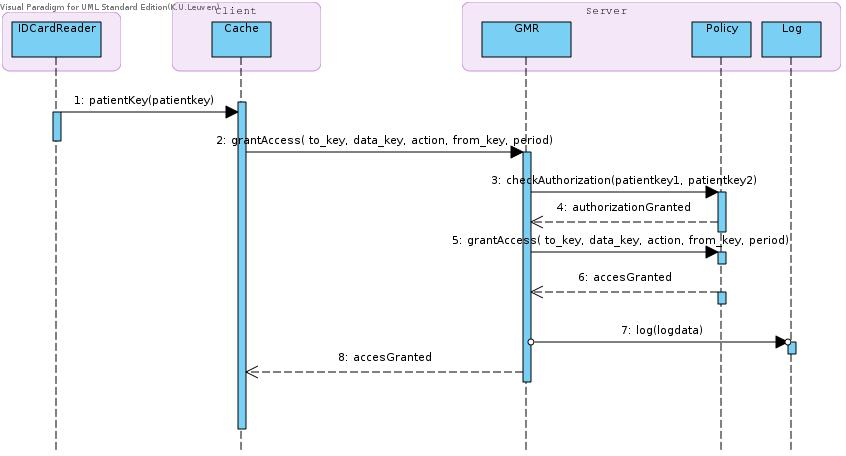
\includegraphics[width=\textwidth]{../images/grantAccess.jpg}
  \caption{Interaction diagram: Grant acces}
\end{figure}

\subsection{Modify GMR}
Wanneer een dokter het dossier van een patient aanpast, doet hij dit eerst op de lokale kopie in zijn cache. De dokter heeft eerst, bij het openen van het dossier, de laatste versie bemachtigd zoals beschreven in het 'access file' diagram. Wanneer hij de wijzigingen hefet opgelagen in zijn cache, worden deze naar de database overgebracht. Er wordt eerst nog gekeken of de dokter ook het recht heeft om te schrijven naar het dossier. Dan worden de wijzigingen opgeslagen in de database. Alle wijzigingen worden op deze manier doorgevoerd, zowel het aanpassen van gegevens, opladen van voorschriften en toevoegen van beeldmateriaal(bv röntgenfotos)\\
Wanneer de server niet bereikbaar blijkt wanneer er veranderingen aan een file worden gemaakt, worden de veranderingen enkel lokaal bijgehouden. Zodra de server weer bereikbaar is, worden de veranderingen doorgevoerd. In principe kan dit leiden tot een inconsistentie (het dossier werd bijgewerkt door iemand anders terwijl de dokter offline was) maar in de praktijk is dit bijna onmogelijk, aangezien een patiënt meestal slechts 1 huisdokter heeft die zijn dossier lokaal bewaart en wanneer andere dokters toch veranderingen aanbrengen (bv een specialist), dan zal dit aan andere velden van het dossier zijn als die dat de dokter heeft aangepast (bv XRay foto's toegevoegd). 

\begin{figure}[!h]
  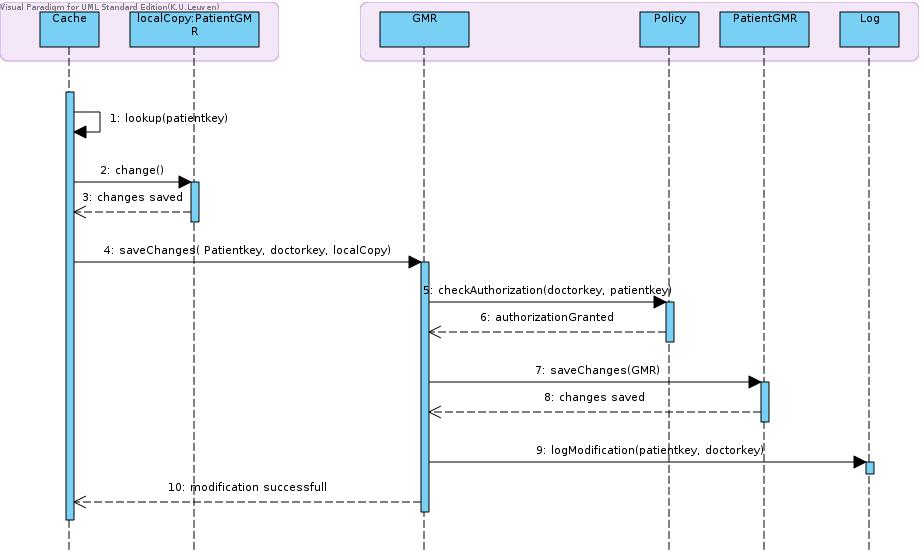
\includegraphics[width=\textwidth]{../images/modifyGMR.jpg}
  \caption{Interaction diagram: Modify GMR}
\end{figure}

\subsection{Retrieve GMR}
Wanneer een dokter een medisch dossier van een patient wilt raadplegen, wordt dit dossier eerst in zijn cache opgezocht. Wanneer het hier gevonden wordt, wordt de timestamp van het dossier in de cache vergeleken met de timestamp van het dossier in de database (indien mogelijk). Wanneer het dossier up to date blijkt, wordt gewerkt met de versie uit de cache. wanneer er aanpassingen zijn geweest, wordt het dossier eerst geupdated in de cache. Wanneer het dossier niet aanwezig blijkt in de cache, wordt het dossier opgehaald en opgeslagen in de cache. 
Deze cache wordt ook gebruikt wanneer de server niet bereikbaar is. Zo kan de dokter toch steeds aan een recente kopie van het dossier van zijn patiënten. Ook de aanpassingen aan de dossiers worden dan enkel lokaal bewaard (zie ook modifyGMR). Zodra de server weer bereikbaar is, worden de veranderingen aan de dossiers ook daar doorgevoerd. 

\begin{figure}[!h]
  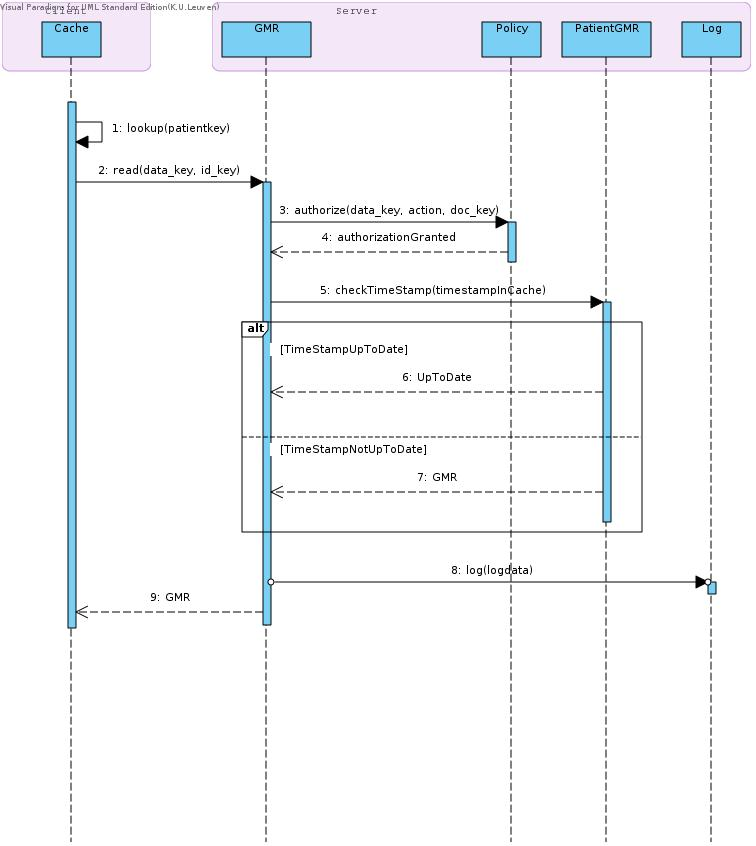
\includegraphics[width=\textwidth]{../images/retrieveGMR.jpg}
  \caption{Interaction diagram: Retrieve GMR}
\end{figure}

\subsection{Add prescription}
\label{interaction:addPrescription}
Wanneer een dokter een voorschrift aan het dossier van een patient koppelt, wordt dit aangepast in het dossier van de patient zoals alle andere wijzigingen.
Het verschil is dat er ook een kopie van het voorschrift op de IDCard van de patient wordt gezet, waarmee deze naar de apotheek kan gaan. 

\begin{figure}[!h]
  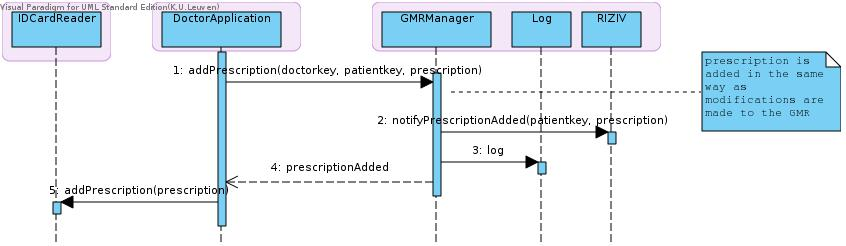
\includegraphics[width=\textwidth]{../images/addprescription.jpg}
  \caption{Interaction diagram: Add prescription}
\end{figure}

\subsection{Validate prescription}
\label{interaction:validatePrescription}
Wanneer de patient naar de apotheek gaat om zijn medicijnen aan te kopen, wordt eerst het voorschrift van zijn IDCard gehaald. De apotheker overhandigd de benodigde medicijnen en duidt zowel op de IDCard als in het systeem aan dat het voorschrift werd gevalideerd. De boodschap naar het Ehealth platform is een boodschap die geen toegang tot het dossier vereist, enkel de key van de apotheker is belangrijk omdat geen andere persoon deze boodschap kan sturen.

\begin{figure}[!h]
  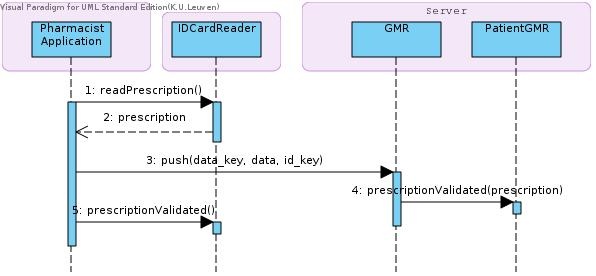
\includegraphics[width=\textwidth]{../images/validatePrescription.jpg}
  \caption{Interaction diagram: Validate prescription}
\end{figure}


\subsection{Architecture background}

Door de bovenvermelde sequentiediagrammen kunnen heel wat acties in het EHealth platform verklaard worden. 
Naast de voor de hand liggende acties (die direct door een sequentiediagram worden aangetoond), zijn ook de volgende scenario's verwezelijkt: 
\paragraph{specialist zendt informatie naar de huisdokter:}
Wanneer een patiënt een specialist consulteert, zal deze tijdelijke toegang krijgen tot het dossier van de patiënt. Hij kan hier dan zijn bevindingen in aanpassen en het dossier opslaan. Wanneer de huisdokter dan het dossier opnieuw opent, kan ook hij deze aanpassingen zien. 

\paragraph{Patiënt bekijkt zijn dossier online:}
Dit is terug te vinden in het diagram retrieve GMR. Wanneer de patiënt Zijn dossier wil bekijken, zal hij zich eveneens aanmelden bij de client applicatie, hier een webapplicatie. Via zijn identificatie gegevens worden de gegevens in het dossier weergegeven die de patiënt mag zien. Wanneer de patiënt zou proberen om wijzigingen aan te brengen in zijn dossier, zal dit niet mogelijk zijn omdat hij de juiste rechten hiervoor niet bezit.

\subsection{Related view packets}
De interactie diagramma's zijn bedoelt om een aantal dingen duidelijk te maken, de architecturale beslissingen staan echter steeds beschreven in de andere views.

\end{document}          
